\documentclass[10pt,twocolumn,letterpaper]{article}
\usepackage[review]{cvpr}
%% This file contains a number of tweaks that are typically applied to the main document.
%% They are not enabled by default, but can be enabled by uncommenting the relevant lines.


%%
%% Official support for 2-column teaser figure
%%
\usepackage{cuted} %< for strip environment

%%
%% For auto-referencing of figures (see fig/teaser.tex and \label{} therein) 
%%
\usepackage{currfile} %< for \currfilebase macro

%%
%% caption and (global) spacing overrides
%%
\usepackage{caption} %< for "\captionof" commands (teaser)
% \setlength{\abovecaptionskip}{.5em} % space above caption
% \setlength{\belowcaptionskip}{1em} % space below caption

%%
%% Inline annotations; for predefined colors, refer to "dvipsnames" in the xcolor package:
%% https://tinyurl.com/overleaf-colors
%%
\newcommand{\red}[1]{{\color{red}#1}}
\newcommand{\todo}[1]{{\color{red}#1}}
\newcommand{\TODO}[1]{\textbf{\color{red}[TODO: #1]}}
%%
%% Disable for camera ready / submission by uncommenting these lines:
%%
% \renewcommand{\TODO}[1]{}
% \renewcommand{\todo}[1]{#1}

%%
%% Work harder in optimizing text layout. Typically shrinks text by 1/6 of page, enable
%% it at the very end of the writing process, when you are just above the page limit.
%%
% \usepackage{microtype}

%%
%% Fine-tune paragraph spacing.
%%
% \renewcommand{\paragraph}[1]{\vspace{.5em}\noindent\textbf{#1.}}

%%
%% Globally adjusts space between figure and caption.
%%
% \setlength{\abovecaptionskip}{.5em}

%%
%% Allows "the use of \paper to refer to the project name"
%% with automatic management of space at the end of the word.
%%
% \usepackage{xspace}
% \newcommand{\paper}{ProjectName\xspace}

%%
%% Commonly used math definitions.
%%
% \DeclareMathOperator*{\argmin}{arg\,min}
% \DeclareMathOperator*{\argmax}{arg\,max}

%%
%% Tighten underline.
%%
% \usepackage{soul}
% \setuldepth{foobar}

%%
%% Reconfigure paragraph (tweaks spacing)
%%

\usepackage{booktabs}
\usepackage{array}
\usepackage{adjustbox}
\usepackage{multirow}
\usepackage{amsmath,amssymb}
\usepackage{graphicx}
\usepackage{xspace}
\newcommand{\ours}{LineageRAFT\xspace}
\newcommand{\rodsim}{\textsc{RodSim}\xspace}
\definecolor{cvprblue}{rgb}{0.21,0.49,0.74}
\usepackage[pagebackref,breaklinks,colorlinks,allcolors=cvprblue]{hyperref}

\def\paperID{*****}
\def\confName{CVPR}
\def\confYear{2027}

\title{Lineage from Two Snapshots, Learned without Lineage Labels\\Supplementary Material}
\author{Anonymous CVPR submission}

\renewcommand{\thetable}{S\arabic{table}}
\renewcommand{\thefigure}{S\arabic{figure}}
\renewcommand{\thesection}{S\arabic{section}}
\begin{document}
\maketitle
\appendix

\section{Implementation details}
\label{sec:supp-impl}
All values are those of our code. OIAM frames are one minute apart; elsewhere $H$ is converted to minutes before entering any model.

\paragraph{\ours tokens.}
From a cell's mask, the eigen-decomposition of its pixel covariance gives the unit major axis $\mathbf{u}$ and standard deviations $\sigma_\parallel\ge\sigma_\perp$.
Let $s$ be the median nearest-neighbour distance among targets, $N_a,N_b$ the counts and $\boldsymbol\mu_a,\boldsymbol\mu_b$ the centroids.
Targets have canonical positions $\tilde{\mathbf{y}}_j=(\mathbf{y}_j-\boldsymbol\mu_b)/s$; ancestors $\tilde{\mathbf{x}}_i=\sqrt{N_b/N_a}(\mathbf{x}_i-\boldsymbol\mu_a)/s$ (radial) or $(\mathcal{A}(\mathbf{x}_i)-\boldsymbol\mu_b)/s$ with $\mathcal{A}$ the Darcy advection; this is also $\mathbf{c}^{(0)}_i$.
The 19-d token concatenates the canonical position (2), $(\mathbf{x}-\text{image centre})/10s$ (2), $(u_y^2{-}u_x^2,2u_yu_x)$ (2), $\log\sigma_\parallel{-}2$ and $\log\sigma_\perp{-}1.4$ (2), $\tanh(\mathbf{b}/4)$ (2) and $\log(1{+}\|\mathbf{b}\|)$ (1) for $\mathbf{b}$ the shortest axis-aligned vector to the image border in units of $s$, the drift $(\boldsymbol\mu_b{-}\boldsymbol\mu_a)/10s$ (2), $[\log_2\frac{H}{60},\log\frac{N_b}{N_a},\log N_a,\log N_b]$ (4) and a one-hot ancestor/target flag (2).
Shape-free models zero the four shape entries.
Augmentation applies one matrix to all vectors: \emph{full}, a rotation $\theta\sim U[0,2\pi)$ then a reflection with probability $\frac12$; \emph{flip}, reflecting $x$ with probability $\frac12$; \emph{none}.

\paragraph{\ours layers} ($d{=}128$, 2{,}875{,}659 parameters).
Input MLPs (one per snapshot): Linear$(19,d)$--GELU--Linear$(d,d)$.
\emph{LocalAttn} is kNN attention with relative-position encoding: queries $W_q\mathrm{LN}(\mathbf{h}^q)$; keys and values $W_{kv}\mathrm{LN}(\mathbf{h}^x)$ gathered at the neighbours plus $\phi(\boldsymbol\delta/4)$, with $\phi$ = Linear$(2,d)$--GELU--Linear$(d,2d)$ of the neighbour offset $\boldsymbol\delta$; 4 heads of 32 channels, softmax over neighbours; residual output projection, then a residual FFN Linear$(d,2d)$--GELU--Linear$(2d,d)$ without normalisation.
\emph{Encoder}: two LocalAttn layers per snapshot over the $k_{\text{self}}{+}1{=}13$ nearest cells (self included) in canonical coordinates.
\emph{GlobalCtx}: $\mathbf{h}\leftarrow\mathbf{h}+\mathrm{MLP}([\mathbf{h},\overline{\mathbf{h}}])$, $\overline{\mathbf{h}}$ the snapshot mean, MLP Linear$(2d,d)$--GELU--Linear$(d,d)$.
\emph{Iteration} $t{=}1..4$ (unshared weights), with $\mathbf{c}=\mathrm{sg}(\mathbf{c}^{(t-1)})$ (stop-gradient):
(i) ancestor $i$ attends to the $k_{\text{cross}}{=}24$ targets nearest $\mathbf{c}_i$, offsets $\tilde{\mathbf{y}}_j{-}\mathbf{c}_i$;
(ii) ancestors attend over their fixed 13-NN graph of initial canonical positions;
(iii) $\mathbf{c}^{(t)}_i=\mathbf{c}_i+\Delta_t(\mathbf{h}_i)$, $\Delta_t$ Linear$(d,2)$ with zero-initialised weight and bias;
(iv) target $j$ attends to its 24 nearest $\mathrm{sg}(\mathbf{c}^{(t)})$, offsets $\mathbf{c}_i{-}\tilde{\mathbf{y}}_j$.
\emph{Assignment}: target $j$ is scored against its $k_{\text{out}}{=}24$ nearest final centres by Linear$(2d{+}3,d)$--GELU--Linear$(d,d)$--GELU--Linear$(d,1)$ on $[\mathbf{h}_j,\mathbf{h}_i,\mathbf{o}/4,\|\mathbf{o}\|/4]$, $\mathbf{o}=\tilde{\mathbf{y}}_j{-}\mathbf{c}^{(T)}_i$ (not detached), plus a dustbin logit Linear$(d,1)(\mathbf{h}_j)$; softmax over 25.
At test time the probabilities are scattered into an $N_b{\times}N_a$ matrix, the dustbin dropped and rows renormalised; no test-time augmentation.
\emph{Family head}: Linear$(2d{+}3,d)$--GELU--Linear$(d,1)$ on $[\mathbf{h}_j,\mathbf{h}_k,\boldsymbol\delta/4,\|\boldsymbol\delta\|/4]$, $\boldsymbol\delta=\tilde{\mathbf{y}}_k{-}\tilde{\mathbf{y}}_j$, logits averaged over both orders.

\paragraph{Labels and losses.}
A target's label is the track alive at $a$ reached through its parents; it is the dustbin if the chain ends at a root born after $a$ or that track has no detection at $a$ (in \rodsim, e.g.\ outside the field of view).
Cross-entropy runs over the 25 classes and ignores targets whose labelled ancestor is not among their candidates.
With $\bar{\mathbf{g}}_i$ the mean canonical position of the labelled descendants of ancestor $i$, $\mathcal{L}_c=\sum_{t=1}^{T}0.8^{T-t}\,\mathrm{mean}_i\min(\|\mathbf{c}^{(t)}_i{-}\bar{\mathbf{g}}_i\|,10)$.
The family loss is a binary cross-entropy for ``same ancestor'' on the directed 8-NN graph of $\tilde{\mathbf{y}}$, restricted to pairs of labelled targets (skipped if fewer than three are labelled).
With $P$ the dense $N_b{\times}(N_a{+}1)$ assignment matrix, dustbin included, the consistency loss on the same pairs is $\mathrm{BCE}(\mathrm{clip}(\sum_iP_{ji}P_{ki},10^{-5},1{-}10^{-5}),[\text{same}])$.
In total, $\mathcal{L}=\mathcal{L}_{\text{CE}}+0.3\mathcal{L}_c+0.5\mathcal{L}_{\text{fam}}+\lambda_{\text{cons}}\mathcal{L}_{\text{cons}}$.

\paragraph{Training.}
A batch is one window: a movie or colony drawn uniformly, $H=\mathrm{round}(\exp U[\ln h_{\min},\ln h_{\max}])$, and a uniform frame $a$ with at least two cells, redrawn until frame $a{+}H$ exists; all cells of both frames are used.
We use AdamW (weight decay 0.01), OneCycle with 5\% warm-up and otherwise PyTorch defaults (cosine, start and end at $1/25$ and $1/(25{\cdot}10^4)$ of the peak, $\beta_1\in[0.85,0.95]$), gradient clipping at norm 1 and bf16 autocast (Table~\ref{tab:impl-raft}).

\begin{table}[t]
\centering\footnotesize\setlength{\tabcolsep}{3pt}
\begin{tabular}{@{}lccc@{}}
\toprule
& OIAM main & \rodsim & fine-tune \\
\midrule
data & M0--M2 & 256 colonies & pseudo-lineage \\
initial weights & random & random & \rodsim \\
steps & 80k & 30k & 6k \\
peak learning rate & $5{\cdot}10^{-4}$ & $5{\cdot}10^{-4}$ & $2{\cdot}10^{-4}$ \\
$h_{\min}$--$h_{\max}$ (min) & 8--240 & 8--240 & 8 or 15--240 \\
$\mathbf{c}^{(0)}$ & Darcy & radial & radial \\
augmentation & none & full & full \\
shape features & yes & no & no \\
$\lambda_{\text{cons}}$ & 0.5 & 0 & 0 \\
seeds & 0, 1, 2 & 0, 1, 2 & 0 \\
\bottomrule
\end{tabular}
\caption{\textbf{\ours settings.} All use $T{=}4$, $k_{\text{self}}{=}12$, $k_{\text{cross}}{=}k_{\text{out}}{=}24$. The annotation-free OIAM model uses the main settings on pseudo-lineage; the ablation without consistency sets $\lambda_{\text{cons}}{=}0$. Fine-tuning: on OIAM $h_{\min}{=}8$, on external sources 15.}
\label{tab:impl-raft}
\end{table}

\paragraph{OIAM evaluation windows.}
With $C{=}66$ frames the median duration of tracks that begin and end with a division in M0--M2, horizons are $\{C/2,C,2C\}$ and anchor frames lie on a grid of step $C/2{=}33$ from the first frame with at least 8 cells, keeping windows with $a{+}H$ within the movie: 20/19/17 windows on M3 and 19/18/16 on M4 at 33/66/132 minutes (109).
Only frames $a$ and $b$ are given (annotated centres in a seeded random order, and mask moments).
The field of interest is the whole image. A target is scored if its chain reaches a track alive and annotated at $a$; descendants of roots born after $a$ (entries), broken chains and unannotated ancestors are excluded.
Accuracy is averaged over windows; \emph{dense} windows have more than 200 ancestors.

\paragraph{Darcy prior.}
With $s_a$ the median nearest-neighbour spacing of ancestors, the grid step is $\ell=\max(s_a/2,2\,\text{px})$ over the image.
For each snapshot, grid cells containing a centre are dilated $r=\max(1,\mathrm{round}(1.5s_a/\ell))$ times, hole-filled and eroded $r{-}1$ times.
We solve $4p_m-\sum_{n\sim m}p_n=g\ell^2$ with $p{=}0$ outside the domain and grid (sparse direct solver); $\mathbf{v}=-\nabla p$ by central differences, interpolated bilinearly.
By default $g=\ln2/68$\,min$^{-1}$ (a fixed doubling time, not fitted). If both snapshots are fully visible (at most 2\% of cells within $2s_a$ of the border), $g=\ln(\max(N_b/N_a,1))/H$ and the result is re-centred on $\boldsymbol\mu_b$; \ours uses this rule, while the ``Darcy 68'' baseline always uses the fixed rate without re-centring and assigns each target to the nearest advected ancestor.
Advection: 12 midpoint (RK2) steps of $H/12$ in $(1{-}\tau)\mathbf{v}_a{+}\tau\mathbf{v}_b$, $\tau$ the elapsed fraction.

\paragraph{Genealogy network} (1{,}291{,}910 parameters).
Pairs are the undirected union of each cell's 8 nearest neighbours.
With $D$ the pair distance, $\varsigma$ a cell's nearest-neighbour distance and $\hat{\mathbf{d}}$ the pair direction, the ten standardised features are $D/\sqrt{\varsigma_j\varsigma_k}$, $D/\sqrt{\sigma_{\parallel j}\sigma_{\parallel k}}$, $|\mathbf{u}_j{\cdot}\mathbf{u}_k|$, $|\hat{\mathbf{d}}{\cdot}\mathbf{u}_j|$, $|\hat{\mathbf{d}}{\cdot}\mathbf{u}_k|$, $|\log\frac{\sigma_{\parallel j}}{\sigma_{\parallel k}}|$, $|\log\frac{\sigma_{\perp j}}{\sigma_{\perp k}}|$, the difference of log aspect ratios, $|\log\frac{\varsigma_j}{\varsigma_k}|$ and the difference of distances to the centroid over their RMS (all absolute).
The z-scored frame is sampled bilinearly on a $64{\times}64$ grid at 1\,px, $x$ axis along the pair, centred on its midpoint; a second channel holds $\exp(-\|\mathbf{p}-\mathbf{p}_c\|^2/0.01)$ at both centres (patch coordinates in $[-1,1]$).
CNN: four stages of [conv$3{\times}3$--BN--ReLU]$\times2$ (32/64/128/256 channels), $2{\times}2$ max-pooling between stages, global average pooling; geometry MLP $10{\to}128{\to}128$; head $384{\to}256{\to}6$ (ReLU).
The outputs are trained with mean binary cross-entropy on $\tau_{jk}<\{8,16,33,66,132,264\}$, $\tau_{jk}$ being $b$ minus the birth frame of the daughter on $j$'s side of the last common ancestor ($10^4$ if none).
Data: M0--M2 frames $250,252,\dots,798$ with at least 8 cells; batches of 4 frames $\times$ 256 pairs; pair order reversed (per frame) and the perpendicular axis reflected (per pair) with probability $\frac12$; AdamW (lr $10^{-3}$, weight decay $10^{-4}$), OneCycle (PyTorch defaults), 15k steps, bf16.
At test time the logits of both orders are averaged and $w_{jk}$ is the sigmoid of the output whose threshold equals $H$; thresholds 8, 16 and 264 are auxiliary targets only.
The annotation-free variant sets $\tau{=}H{-}0.5$ for the smallest threshold $H$ at which both cells chain back to the same pseudo-ancestor.
\emph{Potts decoding}: $q\leftarrow p$ (dustbin removed, renormalised, floored at $10^{-9}$), then 10 synchronous updates $q_j\leftarrow\mathrm{softmax}(\log p_j+\beta\sum_{k\in\mathcal{N}(j)}(2w_{jk}{-}1)q_k)$ on the same graph, without degree normalisation; $\beta{=}2$ (main) or 1 (label-free table).
Ensembles average probabilities before decoding. Windows with fewer than 9 targets or 2 ancestors are not decoded.

\paragraph{\rodsim.}
Cells are spherocylinders (cap radius $r{=}0.5\,\mu$m, length $L$, angle $\theta$), each represented by $\max(2,\lceil(L{-}2r)/r\rceil{+}1)$ spheres along its axis. Every minute:
(1) $L\leftarrow Le^{\lambda}$, $\lambda=\frac{\ln2}{T_d}e^{\epsilon}$, $\epsilon\sim\mathcal{N}(0,\mathrm{CV}_g^2)$ drawn at birth;
(2) adder division when $L{-}L_{\text{birth}}\ge\ell_0e^{\eta}$, $\eta\sim\mathcal{N}(0,\mathrm{CV}_a^2)$ drawn at birth: the septum sits at fraction $f=\mathrm{clip}(\frac12{+}\mathcal{N}(0,\sigma_f^2),0.3,0.7)$ and daughters of lengths $fL,(1{-}f)L$ lie on either side along $\theta\mp\varsigma\alpha/2+\mathcal{N}(0,\sigma_\theta^2)$, $\varsigma{=}\pm1$, $\alpha=|\mathcal{N}(0,(1.2533\bar\alpha)^2)|$ (mean $\bar\alpha$); widths inherit a factor $e^{\mathcal{N}(0,\mathrm{CV}_w^2)}$;
(3) eight sub-steps in which spheres of different cells closer than $2r$ repel with force $2r{-}d$, giving per cell $\Delta\mathbf{x}=(\kappa\mathbf{F}_\parallel{+}\mathbf{F}_\perp)/2L$ and $\Delta\theta=M/(L^3/12)$ for net force $\mathbf{F}$ and torque $M$;
(4) $\Delta\mathbf{x}\sim\mathcal{N}(0,D^2I)$, $\Delta\theta\sim\mathcal{N}(0,D_r^2)$.
Founders: positions $\mathcal{N}(0,(2\,\mu\text{m})^2I)$, $\theta\sim U[0,\pi)$, $L=\ell_0U(1,1.9)$, $L_{\text{birth}}=L/U(1,1.9)$.
Colonies stop at $N_{\max}$ cells or 1{,}500 minutes; every minute is recorded with $\sigma_\parallel=L/\sqrt{12}$, $\sigma_\perp=wr/2$.
\emph{Field of view}: with $R$ = 1.4$\times$ the final RMS radius ${+}1\,\mu$m, a square of half-side $\rho R$ centred at the final centroid ${+}\,\mathbf{o}R$, at $\gamma$ px/$\mu$m; cells outside are dropped, ancestry uses the full tree.
Division modes add per-frame noise $e^{\mathcal{N}(0,\sigma_{\text{obs}}^2)}$ on $\sigma_\parallel,\sigma_\perp$ and $\mathcal{N}(0,\sigma_{\text{ang}}^2)$ on the axis (Table~\ref{tab:impl-rodsim}). Colony seeds are $0..255$.
\emph{Rendering} (\rodsim genealogy; 6 frames per colony at minute $\ge$200 with 30--1{,}500 cells, 200 colonies): rescale so that the width $4\,\mathrm{median}\,\sigma_\perp$ is $U(12,19)$\,px; draw capsules of radius $2\sigma_\perp$ through their signed distance, blending background $U(0.6,1)$ and cell level $U(0,0.3)$ by $\mathrm{sigmoid}(-\mathrm{sdf}/U(0.5,1.5))$, with per-cell factor $1{+}\mathcal{N}(0,U(0,0.15)^2)$; add an outside halo (amplitude $U(0,0.6)$, decay $U(1,4)$\,px), a linear gradient $\mathcal{N}(0,0.15^2)$ per axis, Gaussian blur $U(0.7,2)$\,px and noise of s.d.\ $U(0.01,0.08)$.
Render v2 instead inherits the per-cell factor from the mother times $e^{\mathcal{N}(0,U(0.03,0.12)^2)}$ and constricts the longest $U(5,25)\%$ of cells at mid-cell (depth $U(0.15,0.45)r$, width $0.6r$). Image patches are also z-scored per patch.

\begin{table}[t]
\centering\footnotesize\setlength{\tabcolsep}{3pt}
\begin{tabular}{@{}llc@{}}
\toprule
parameter & range (uniform) & midpoint \\
\midrule
birth length $\ell_0$ & 1--3\,$\mu$m & 2 \\
doubling time $T_d$ & 40--110\,min & 75 \\
growth-rate CV$_g$ & 0.05--0.3 & 0.15 \\
adder CV$_a$ & 0.05--0.25 & 0.15 \\
division angle noise $\sigma_\theta$ & 0--0.15\,rad & 0.07 \\
position noise $D$ & 0--0.02\,$\mu$m/min & 0.01 \\
angle noise $D_r$ & 0--0.03\,rad/min & 0.015 \\
drag anisotropy $\kappa$ & 0.5--2 & 1 \\
founders $n_0$ & 1--4 & -- \\
final cells $N_{\max}$ & 900--2199 & -- \\
pixel scale $\gamma$ & 6--14\,px/$\mu$m & -- \\
FOV half-size $\rho$ & 0.35--1.2 & -- \\
FOV offset $\mathbf{o}$ (per axis) & $-$0.4--0.4 & -- \\
\midrule
\multicolumn{3}{@{}l}{\emph{division modes only (otherwise 0)}}\\
septum s.d.\ $\sigma_f$ & 0--0.08 & -- \\
mean V-snap angle $\bar\alpha$ & 0--1.2\,rad & -- \\
width CV$_w$ & 0--0.06 & -- \\
length/width noise $\sigma_{\text{obs}}$ & 0--0.08 & -- \\
axis noise $\sigma_{\text{ang}}$ & 0--0.15\,rad & -- \\
\bottomrule
\end{tabular}
\caption{\textbf{\rodsim randomisation}, drawn once per colony (integers for $n_0,N_{\max}$). Midpoints: fixed-physics ablation.}
\label{tab:impl-rodsim}
\end{table}

\paragraph{Self-labelling.}
For frames $t\to t{+}1$, each cell of $t$ offers a \emph{stay} slot at $\mathbf{x}_i$ and two daughter slots at $\mathbf{x}_i\pm\frac{L_i}{4}\mathbf{u}_i$ ($L_i=\sqrt{12}\sigma_{\parallel i}$), and each cell of $t{+}1$ a private no-parent column.
Costs are Euclidean distances, plus 10\,px for daughter slots; no parent costs 60\,px; only the 8 nearest slots of each type are finite.
Each cell of $t{+}1$ is matched to one column by exact linear assignment (SciPy); a slot takes one cell, so a parent can take up to three.
Without masks, daughter slots sit at $\mathbf{x}_i$, the extra cost is $0.55s$ and no parent $3.5s$ ($s$ the median nearest-neighbour spacing of frame $t$).
Pseudo-ancestry composes links backwards; a no-parent link gives the dustbin.
\emph{Temporal bootstrapping} replaces each link by the argmax (dustbin excluded) of the \rodsim model on $(t,t{+}1)$, positions only, with $H$ the frame interval.
For adaptation, each source's sequences, sorted by name, alternate between two folds; a model fine-tuned on one fold is tested on the other.

\paragraph{Per-colony processing and SV.}
Ancestors are grouped by single linkage at 3 median spacings; targets join the colony of their nearest ancestor; the \rodsim model runs per colony (a one-ancestor colony takes all its targets).
SV scores nearest assignment and per-colony \ours by \emph{coverage}, the fraction of ancestors receiving at least one target (all targets counted), and keeps the higher; ties go to the lower coefficient of variation of family sizes (zeros included), then to nearest assignment.
External inputs are positions only, with image size $1.05\times$ the detections' bounding box ${+}5$\,px.

\paragraph{Compute.}
Training ran on one shared NVIDIA H200: 1.9--3.0\,h per 80k-step OIAM model, 0.6--1.2\,h per 30k-step \rodsim model, about 13\,min per 6k-step fine-tune; 19\,min for the OIAM genealogy network (15k steps) and about 41\,min for the \rodsim one, including rendering.


\section{What family registration needs}
\label{sec:core}
\cref{tab:core} isolates the family centre. At a fixed budget of 30k steps, accuracy rises with the number of refinement rounds (0.79, 0.83, 0.86 and 0.88 at 33 minutes for $T{=}0,1,2,4$), and keeping all four attention rounds but freezing the centre (the direct matcher) falls back to the level of the matcher without cross-attention, most clearly on dense windows (0.63 \vs 0.77 at 33 minutes, 0.36 \vs 0.47 at 66). The gain is largest at short and medium gaps and small at 132 minutes (0.419 \vs 0.424), where the partition limits accuracy. The training logs show that the true ancestor is among a target's 24 candidates for 99\% of training targets with a moving centre and for 95\% with a fixed one; the controls below show that this is not the explanation. Longer training matters as much as the architecture: the same model (seed 0) reaches 0.877 at 33 minutes after 30k steps and 0.962 after 80k. Longer training does not close the gap. In a second protocol, fixed before training, we trained the direct matcher at the main-table budget (80k steps, three seeds) with Darcy and with radial initialisation, and compared seed-mean accuracy per window. With Darcy initialisation, \ours is ahead by 0.101 [0.068, 0.138], 0.096 [0.072, 0.123] and 0.017 [0.004, 0.031] at 33/66/132 minutes, and on dense windows by 0.201, 0.169 and 0.061, winning every dense window at every gap (hypotheses D1, D2 hold). With radial initialisation it is ahead by 0.102 and 0.068 at 33 and 66 minutes but ties at 132 ($-$0.005 [$-$0.027, 0.019]; D3 fails there), although it still leads on dense windows (0.069 [0.030, 0.108]). Candidate recall in training stays at 0.95--0.96 for the direct matcher and 0.997 for \ours after 80k steps. A third protocol, also fixed before training (three seeds each, Darcy initialisation, 80k steps), tested three simpler explanations of the gap. (K1)~Four times as many candidates (96) restore the direct matcher's recall to 0.99 but its accuracy only to 0.868/0.696/0.458; \ours stays ahead by 0.089 [0.062, 0.117] and 0.084 [0.067, 0.102] at 33 and 66 minutes, so missing candidates are not the cause. (K2)~Training the centre head with the centre loss but never using it gives 0.904/0.709/0.457: centre supervision as an auxiliary task explains about half of the gain at 33 minutes and little at 66 (\ours ahead by 0.053 [0.026, 0.085] and 0.071 [0.044, 0.100]). (K3)~One refinement round instead of four, with the same full recall, gives 0.873/0.670/0.450 (\ours ahead by 0.083 [0.062, 0.107] at 33 minutes). All three hypotheses hold, and \ours wins every dense window against every control at every gap; at 132 minutes the differences are 0.015--0.023. What matters is that candidates are scored relative to a centre that has moved over several rounds, not which ancestors are in the candidate set.
\begin{table}[t]
\centering\small
\setlength{\tabcolsep}{3pt}
\begin{adjustbox}{max width=\linewidth}
\begin{tabular}{lcccccc}
\toprule
 & \multicolumn{3}{c}{All windows} & \multicolumn{3}{c}{Dense ($>$200)} \\
\cmidrule(lr){2-4}\cmidrule(lr){5-7}
Model & 33 & 66 & 132 & 33 & 66 & 132 \\
\midrule
\multicolumn{7}{l}{\emph{30k steps, seed 0 (core ablation)}} \\
$T{=}4$, moving centre (reference) & .877 & .663 & .424 & .773 & .469 & .208 \\
$T{=}2$ & .858 & .664 & .431 & .732 & .467 & .217 \\
$T{=}1$ & .825 & .648 & .422 & .681 & .435 & .206 \\
$T{=}0$: learned pairwise matcher & .790 & .620 & .416 & .653 & .405 & .196 \\
$T{=}4$, fixed centre (direct matcher) & .806 & .623 & .419 & .631 & .364 & .191 \\
\multicolumn{7}{l}{\emph{80k steps, mean of three seeds (matched direct matcher)}} \\
\ours, Darcy init. & .957 & .780 & .473 & .907 & .598 & .267 \\
Direct matcher, Darcy init. & .856 & .684 & .456 & .706 & .429 & .207 \\
\ours, radial init. & .948 & .748 & .454 & .894 & .567 & .275 \\
Direct matcher, radial init. & .846 & .681 & .458 & .685 & .433 & .206 \\
Direct matcher, 96 candidates & .868 & .696 & .458 & .736 & .475 & .229 \\
Direct matcher + centre loss & .904 & .709 & .457 & .789 & .445 & .205 \\
\ours, $T{=}1$ & .873 & .670 & .450 & .756 & .466 & .233 \\
\multicolumn{7}{l}{\emph{80k steps, seed 0}} \\
\ours without consistency term & .963 & .789 & .478 & .918 & .618 & .269 \\
\ours, $T{=}8$ & .941 & .750 & .441 & .885 & .582 & .237 \\
\bottomrule
\end{tabular}
\end{adjustbox}
\caption{\textbf{What family registration needs} (OIAM M3/M4, accuracy, argmax). All rows use shape features, no rotation augmentation and the consistency term; Darcy initialisation unless stated. $T$: rounds of cross-snapshot attention and centre update. With $T{=}0$ each snapshot is encoded on its own and targets are scored against the initial anchor positions, a learned pairwise matcher. The direct matcher is the same network with the same 2.9M parameters, data, losses and schedule, except that the family centre never moves and has no loss: targets cross-attend to, and are scored against, candidate ancestors at their initial positions. Controls: the direct matcher with 96 instead of 24 candidate ancestors per target, or with the centre head trained by the centre loss but never used. All three protocols were fixed before training and run once.}
\label{tab:core}
\end{table}


\paragraph{How do the centres move?}
\cref{fig:centretraj} follows the family centres of the full model (seed 0) through the four rounds on M3/M4.
The first round removes most of the initial error and later rounds keep reducing it: on dense windows the mean distance to the true family centroid falls from 2.1 to 0.3 cell spacings at 33 minutes, from 3.7 to 1.3 at 66 minutes and from 6.5 to 3.1 at 132 minutes, and the true ancestor is among a target's 24 nearest centres for 0.99/0.97/0.90 of targets instead of 0.90/0.78/0.69 at initialisation.
Candidate recall alone does not explain the gain: the direct matcher with 96 candidates reaches 0.99 recall in training and still trails by 0.08--0.09 at 33 and 66 minutes (\cref{tab:core}). What helps is that target offsets are measured from a point close to the family.
Accuracy follows the centre: targets whose family centre ends within half a spacing of the true centroid are assigned correctly in 0.98/0.89/0.62 of cases at 33/66/132 minutes, beyond four spacings in 0.05--0.07. Larger families are harder: at 132 minutes accuracy is 0.35, 0.33 and 0.25 for families of 2, 3--4 and 5--8 scored descendants (rare unsplit cells: 0.12).
\paragraph{On small colonies the centre adds little.}
Under a protocol fixed before training (\texttt{docs/vv\_family\_vs\_direct\_protocol.md}) we repeated the bootstrapped self-labelling of blind test 4 (main-text Table 5) with the direct matcher: initialised from the \rodsim direct matcher, trained on the same pseudo-lineage of the other fold with the same settings, and evaluated on the same windows of the 28 van Vliet colonies.
Self-labelling helps both equally (0.660$\to$0.698 for \ours, 0.655$\to$0.695 for the direct matcher), and \ours leads by only 0.003 [$-$0.001, 0.007] over colonies (17 of 28 colonies; ahead in all three subsets by 0.002--0.005): the primary hypothesis, a CI above zero, fails.
These windows are small (median 10 ancestors, 99th percentile 186, against more than 200 for a dense OIAM window); post hoc, in the 188 windows with more than 100 ancestors at 30 minutes \ours leads by 0.028 [0.023, 0.033] (window bootstrap), and by at most 0.004 elsewhere.
The same holds on OIAM (post hoc, \texttt{experiments/centre\_crowding\_analysis.py}): the full model's margin over the direct matcher grows with the number of ancestors in a window (Spearman $\rho$ 0.88/0.88/0.69 at 33/66/132 minutes), from 0.02/0.02/$-$0.01 in windows of at most 25 ancestors to 0.24/0.19/0.08 in windows of more than 400.
The moving family centre is thus a remedy for crowding: it matters where many families compete for each target, as in dense OIAM windows, and not in microcolonies, where a learned matcher does as well.

\begin{figure*}[t]
\centering
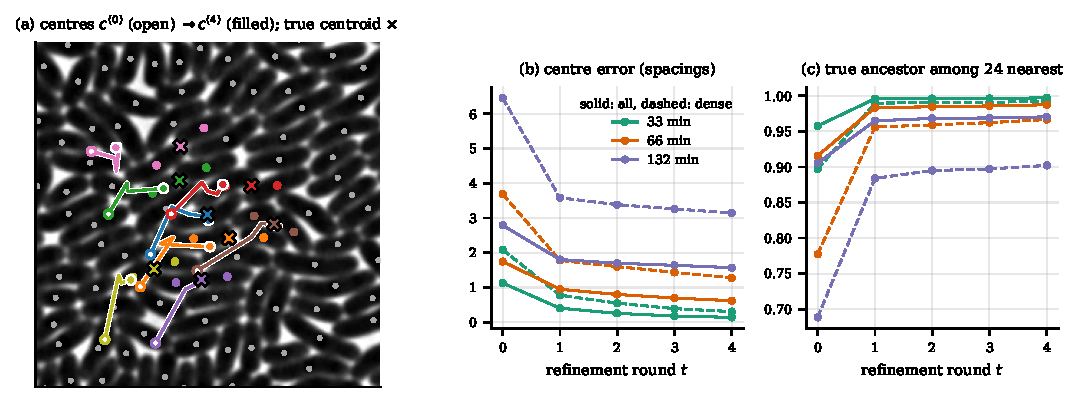
\includegraphics[width=0.95\linewidth]{fig/centre_trajectory.pdf}
\caption{\textbf{Family centres through the refinement rounds.} (a) The eight families nearest the centre of a crop of a dense 66-minute OIAM window (the window of the qualitative figure) among those whose initial (Darcy) centre is more than 1.5 spacings off; dots: their scored descendants. (b) Mean distance from each ancestor's centre to its true family centroid, in target cell spacings, after round $t$ ($t{=}0$: initialisation). (c) Fraction of targets whose true ancestor is among the 24 centres nearest to them, the candidate set of the assignment step. Solid: all M3/M4 windows; dashed: dense windows ($N_a{>}200$).}
\label{fig:centretraj}
\end{figure*}

\section{All in-domain variants}
\cref{tab:oiamfull} extends Table~2 of the main paper with Trackastra's greedy decoding, the rotation-augmented model with Darcy initialisation, the full model with the genealogy decoder, and the undecoded three-seed ensemble.
\begin{table}[t]
\centering\small
\setlength{\tabcolsep}{3.5pt}
\begin{adjustbox}{max width=\linewidth}
\begin{tabular}{lcccccc}
\toprule
& \multicolumn{3}{c}{All windows} & \multicolumn{3}{c}{Dense ($N_a{>}200$)} \\
\cmidrule(lr){2-4}\cmidrule(lr){5-7}
Method & 33 & 66 & 132 & 33 & 66 & 132 \\
\midrule
Nearest ancestor & .497 & .361 & .263 & .157 & .083 & .058 \\
Radial expansion & .547 & .458 & .342 & .249 & .154 & .056 \\
Darcy flow prior (ours) & .627 & .466 & .368 & .305 & .161 & .088 \\
Optical flow (RAFT~\cite{teed2020raft}) & .636 & .367 & .244 & .347 & .094 & .041 \\
Unbalanced OT~\cite{schiebinger2019optimal} & .555 & .473 & .353 & .257 & .159 & .056 \\
Non-rigid CPD~\cite{myronenko2010cpd} & .597 & .466 & .359 & .294 & .162 & .060 \\
Family-centre regression (GBDT) & .731 & .610 & .446 & .449 & .297 & .201 \\
Trackastra~\cite{gallusser2024trackastra}, greedy & .670 & .239 & .215 & .366 & .079 & .062 \\
Trackastra~\cite{gallusser2024trackastra}, argmax & .681 & .176 & .162 & .395 & .073 & .057 \\
Trackastra, fine-tuned per gap & .892 & .716 & .451 & .788 & .507 & .171 \\
Trackastra, fine-tuned over gaps & .864 & .700 & .488 & .739 & .476 & .230 \\
Trackastra, fine-tuned$^\dagger$ & .892 & .716 & .488 & .788 & .507 & .230 \\
\ours, rot.\ aug. & .741 & .604 & .451 & .459 & .294 & .178 \\
\ours, no rot. & .853 & .653 & .447 & .717 & .443 & .247 \\
\ours, rot.\ aug. + Darcy init & .795 & .692 & .511 & .557 & .397 & .222 \\
Direct matcher (\ours, fixed centre) & .856 & .684 & .456 & .706 & .429 & .207 \\
\ours, full & .957 & .780 & .473 & .907 & .598 & .267 \\
\ours, full recipe, M0/M1 only, 20k steps & .715 & .554 & .394 & .501 & .289 & .154 \\
\ours, full + genealogy decoder & .966 & .814 & .485 & .928 & .650 & .275 \\
\ours, 3-seed ensemble & .964 & .807 & .490 & .923 & .634 & .284 \\
\ours, ensemble + decoder & \textbf{.977} & \textbf{.863} & \textbf{.517} & \textbf{.946} & \textbf{.703} & \textbf{.300} \\
\ours, ensemble + decoder, no annotation & .963 & .822 & .487 & .919 & .634 & .260 \\
\midrule
\textcolor{gray}{Oracle family partition} & .984 & .929 & .784 & .963 & .817 & .465 \\
\bottomrule
\end{tabular}
\end{adjustbox}
\caption{\textbf{In-domain results on OIAM M3/M4} (trained on M0--M2). Accuracy at gaps of 33/66/132 minutes. Trackastra receives images and ground-truth masks of both snapshots. $^\dagger$Fine-tuned on M0/M1 lineage, one model per gap or one over five gaps, whichever is better on M2 (per gap at 33/66, over gaps at 132 minutes; checkpoint and decoding also chosen on M2). M3/M4 were inspected during development (leave-one-movie-out: supplement). Direct matcher: the same network with the family centre frozen at its initial position. Rot.\ aug./no rot.: 30k steps, radial initialisation, with/without rotation augmentation; full: see text. Direct matcher and full (and its decoder row): mean of 3 seeds (std $\le$0.016); ensemble rows average the seeds' probabilities; no annotation: both networks trained on self-labelled lineage of the unannotated M0--M2; oracle: ensemble; other learned rows: one seed.}
\label{tab:oiamfull}
\end{table}


\section{Leave-one-movie-out evaluation}
OIAM M3/M4 were inspected during development. \cref{tab:lomo} trains on four OIAM movies and tests on the fifth, for all five folds.
The full model, retrained in each fold under a protocol fixed beforehand (\texttt{docs/full\_lomo\_protocol.md}), reaches 0.954/0.792/0.483 on average over held-out movies, against 0.957/0.780/0.473 on the M3/M4 test: the development test movies did not flatter it. All three hypotheses hold: it beats the 30k-step no-rotation model at 33 and 66 minutes and the regressor at every gap on all five folds, and averages at least 0.90 at 33 minutes. On dense windows it averages 0.90/0.60/0.26.
\begin{table}[t]
\centering\small
\setlength{\tabcolsep}{3pt}
\begin{adjustbox}{max width=\linewidth}
\begin{tabular}{lccccccccc}
\toprule
& \multicolumn{3}{c}{Family-centre regression} & \multicolumn{3}{c}{\ours, no rot., 30k} & \multicolumn{3}{c}{\ours, full} \\
\cmidrule(lr){2-4}\cmidrule(lr){5-7}\cmidrule(lr){8-10}
Held out & 33 & 66 & 132 & 33 & 66 & 132 & 33 & 66 & 132 \\
\midrule
M0 & .724 & .582 & .408 & .884 & .697 & .436 & \textbf{.955} & \textbf{.748} & \textbf{.447} \\
M1 & .777 & .650 & .451 & .900 & .721 & .487 & \textbf{.955} & \textbf{.824} & \textbf{.518} \\
M2 & .698 & .556 & .409 & .834 & .631 & .440 & \textbf{.928} & \textbf{.764} & \textbf{.451} \\
M3 & .738 & .599 & .434 & .859 & .630 & .422 & \textbf{.964} & \textbf{.793} & \textbf{.489} \\
M4 & .724 & .622 & .459 & .849 & .690 & .453 & \textbf{.966} & \textbf{.830} & \textbf{.511} \\
\midrule
Mean & .732 & .602 & .432 & .865 & .674 & .447 & \textbf{.954} & \textbf{.792} & \textbf{.483} \\
\bottomrule
\end{tabular}
\end{adjustbox}
\caption{\textbf{Leave-one-movie-out on OIAM.} Each row trains on the other four movies and tests on all windows of the held-out one. \ours, full: the configuration of the main results (80k steps, Darcy initialisation, consistency term, no rotation), one seed, fixed before running (protocol in the ledger). The five movies come from one experiment, so folds measure sensitivity to the movie, not independent replication. Bold: the best model per gap.}
\label{tab:lomo}
\end{table}


\paragraph{Does the no-rotation gain need the chamber orientation?}
In-domain OIAM models are trained without rotation augmentation, which exploits the fixed orientation of the growth chambers in the image. We tested whether this prior must be known (\texttt{docs/orientation\_protocol.md}): each M3/M4 window is presented in all eight orientations and reflections of the image (positions, cell axes, image borders and Darcy initialisation transformed exactly). Without correction, the no-rotation model (three-seed mean) drops from 0.957/0.780/0.473 to 0.851/0.689/0.421 (dense 0.907/0.598/0.267 to 0.649/0.359/0.125), close to the rotation-augmented model (0.807/0.698/0.510 over the eight frames). The chamber axis can be estimated per sequence without labels from the sign of the nematic order $\langle\cos 2\phi\rangle$ of the cells' major axes (chosen on M0--M2; correct for both test sequences in all eight frames), leaving four axis-preserving frames. The rule fixed as primary before the test, which picks among these the frame with the highest model confidence, gives 0.942/0.764/0.465 (dense 0.873/0.556/0.236), recovering 90\% and 80\% of the no-rotation gain over the rotation-augmented model at 33 and 66 minutes; at 132 minutes there is no gain to recover over all windows. Averaging the predictions of the four frames, the rule we had planned first but replaced after a design check on the training movies, recovers all of it (0.962/0.813/0.504; dense 0.910/0.602/0.247). The orientation prior is therefore a property of the experiment that can be estimated from the detections, not knowledge supplied by the user.

\section{Uncertainty, weighting and paired tests}
\cref{tab:reliability} adds 95\% bootstrap intervals over windows to the main table and weights the same predictions by targets.
Weighting by targets lowers every method, most at long gaps, because dense windows are hardest; the ranking is unchanged.
Window intervals are wide because windows differ in density, but paired comparisons over the same windows are tight.
At 132 minutes the full model beats the family-centre regressor by 0.027 (95\% CI 0.003--0.048; 25 of 33 windows), the ensemble with decoder by 0.071 (0.044--0.094; 29 of 33) and the annotation-free pipeline by 0.041 (0.018--0.062; 26 of 33).
Ensembling and decoding improve the full model at every gap (+0.021/+0.083/+0.044, all intervals above 0.009), and annotation-free training costs 0.014/0.042/0.030 (intervals 0.009--0.019, 0.029--0.054, 0.012--0.047).
\begin{table}[t]
\centering\small
\setlength{\tabcolsep}{3pt}
\begin{adjustbox}{max width=\linewidth}
\begin{tabular}{lcccccc}
\toprule
& \multicolumn{3}{c}{Window-averaged (95\% CI)} & \multicolumn{3}{c}{Cell-weighted} \\
\cmidrule(lr){2-4}\cmidrule(lr){5-7}
Method & 33 & 66 & 132 & 33 & 66 & 132 \\
\midrule
Nearest ancestor & .497{\scriptsize$\pm$.104} & .361{\scriptsize$\pm$.092} & .263{\scriptsize$\pm$.070} & .183 & .113 & .098 \\
Unbalanced OT & .555{\scriptsize$\pm$.093} & .473{\scriptsize$\pm$.090} & .353{\scriptsize$\pm$.079} & .244 & .178 & .138 \\
Non-rigid CPD & .597{\scriptsize$\pm$.093} & .466{\scriptsize$\pm$.091} & .359{\scriptsize$\pm$.076} & .268 & .179 & .143 \\
Trackastra, fine-tuned per gap & .892{\scriptsize$\pm$.037} & .716{\scriptsize$\pm$.064} & .451{\scriptsize$\pm$.073} & .762 & .502 & .243 \\
Family-centre regression (GBDT) & .731{\scriptsize$\pm$.083} & .610{\scriptsize$\pm$.092} & .446{\scriptsize$\pm$.075} & .440 & .321 & .255 \\
\ours, full (mean of 3 seeds) & .957{\scriptsize$\pm$.019} & .780{\scriptsize$\pm$.053} & .473{\scriptsize$\pm$.060} & .895 & .599 & .317 \\
\ours, ensemble + decoder & .977{\scriptsize$\pm$.014} & .863{\scriptsize$\pm$.050} & .517{\scriptsize$\pm$.062} & .937 & .698 & .353 \\
\ours, no annotation & .963{\scriptsize$\pm$.018} & .822{\scriptsize$\pm$.053} & .487{\scriptsize$\pm$.070} & .908 & .636 & .311 \\
\midrule
\textcolor{gray}{Oracle family partition} & .984{\scriptsize$\pm$.011} & .929{\scriptsize$\pm$.039} & .784{\scriptsize$\pm$.080} & .954 & .804 & .560 \\
\bottomrule
\end{tabular}
\end{adjustbox}
\caption{\textbf{Uncertainty and weighting} on OIAM M3/M4. Left: accuracy averaged over windows (as in the main table) with the half-width of a 95\% bootstrap interval over windows. Right: the same predictions weighted by scored targets, which counts the dense windows more. Decoder rows use the windows with at least 9 targets.}
\label{tab:reliability}
\end{table}


\paragraph{Quality of the uncurated recA and rpsM lineages.}
Unlike FAST, recA and rpsM carry uncurated Schnitzcells lineages, so we audited them against FAST with statistics fixed in advance (\texttt{docs/schnitzcells\_audit\_protocol.md}), on exactly the scored targets.
Neither contains non-binary divisions, interior orphans or lost cells.
Size changes at division and large displacements are flagged often (76\% and 9\% of scored recA and rpsM targets lie on a flagged lineage path), but almost all flags are explained by one frame of growth (7.5 minutes) and whole-colony stage drift; after correcting for both (post hoc), 5.2\% (recA) and 1.7\% (rpsM) of scored targets lie on a flagged path, against 0.2\% on FAST.
Label errors on a fraction $f$ of targets shift a method difference by at most $2f$; only the extreme case for recA (all flagged labels wrong, all in favour of the baseline) reaches its 0.10 margin.
The margin over each colony's best geometric baseline is positive in all 25 colonies, unchanged in colonies with few flags, and of similar size on curated FAST, so label noise does not explain the zero-shot result; swaps of two adjacent cells of similar size would escape these checks.

\section{Optimal-transport and registration baselines}
\cref{tab:ot} lists all six optimal-transport variants.
Transport with uniform growth spreads every ancestor's mass over its neighbourhood: it fixes the most blatant failure of nearest assignment, interior ancestors receiving no target, but cannot know which ancestors grew or where the colony flowed, so in dense windows it stays below 0.30 even at 33 minutes, against 0.91 for \ours.
\begin{table}[t]
\centering\small
\setlength{\tabcolsep}{3pt}
\begin{adjustbox}{max width=\linewidth}
\begin{tabular}{lcccccc}
\toprule
& \multicolumn{3}{c}{All windows} & \multicolumn{3}{c}{Dense ($N_a{>}200$)} \\
\cmidrule(lr){2-4}\cmidrule(lr){5-7}
Coupling, alignment & 33 & 66 & 132 & 33 & 66 & 132 \\
\midrule
Exact capacity, none & .545 & .506 & .360 & .217 & .215 & .079 \\
Exact capacity, radial & .549 & .476 & .352 & .251 & .158 & .056 \\
Exact capacity, darcy & .560 & .492 & .372 & .285 & .197 & .093 \\
Entropic unbalanced, none & .561 & .445 & .337 & .225 & .112 & .073 \\
Entropic unbalanced, radial & .555 & .473 & .353 & .257 & .159 & .056 \\
Entropic unbalanced, darcy & .564 & .491 & .376 & .298 & .189 & .102 \\
\bottomrule
\end{tabular}
\end{adjustbox}
\caption{\textbf{Optimal-transport baselines} on OIAM M3/M4. Hyperparameters (capacity factor; entropy and KL relaxation) chosen on M0--M2. Costs are squared distances in units of the ancestor spacing.}
\label{tab:ot}
\end{table}

Non-rigid CPD~\cite{myronenko2010cpd} treats ancestors as the centroids of a Gaussian mixture, moves them with a Gaussian-kernel displacement field of width $\beta$ and regularisation $\lambda$ (coordinates in ancestor spacings, 150 EM iterations), and assigns each target to the centroid of highest posterior.
We searched $\beta\in\{2,4,8,16,32\}$, $\lambda\in\{1,4,16\}$, outlier weight $w\in\{0,0.1\}$, with or without radial pre-alignment, on M0--M2; the selected setting ($\beta{=}8$, $\lambda{=}4$, $w{=}0$, radial) is interior to the grid, and its grid neighbours score within 0.007 on M0--M2.
On M3/M4 it reaches 0.597/0.466/0.359 (dense 0.294/0.162/0.060), the level of unbalanced OT: a smooth deformation cannot follow the many independent family displacements of a dense colony.

\paragraph{Trackastra fine-tuned at each gap.}
The public \texttt{general\_2d} model never saw gaps of an hour or more, so we also fine-tune it in domain, following a protocol fixed before training (one model per gap; architecture, features, loss, augmentation and optimiser of the official training script; batch 8 instead of 48 for memory; 20k steps).
Training data are M0/M1 subsampled at the gap from every start frame, each detection's parent being its ground-truth ancestor one subsampled frame earlier, with images and ground-truth masks; the checkpoint (every 1k steps) and the decoding are chosen on M2, and M3/M4 are evaluated once.
M2 accuracy rises from 0.66/0.16/0.17 off the shelf to 0.86/0.67/0.43; at 132 minutes it peaks at the first checkpoint and then declines while the training loss keeps falling, so that checkpoint is used.
Argmax beats the greedy linker on M2 at every gap; on M3/M4 the greedy linker reaches 0.870/0.667/0.340 (dense 0.731/0.415/0.062) and argmax 0.892/0.716/0.451 (dense 0.788/0.507/0.171; main-text table at 33/66 minutes).
Paired over windows, \ours (mean of three seeds) exceeds it by 0.065 [0.045, 0.087], 0.064 [0.043, 0.087] and 0.023 [$-$0.003, 0.048] at 33/66/132 minutes and wins every dense window at every gap; the ensemble with decoder exceeds it by 0.088/0.148/0.067, and the pipeline without annotation by 0.074/0.106/0.036 (all intervals above zero), winning every dense window at every gap.
Fine-tuning closes most of the gap to \ours at 33 minutes but not in dense colonies (0.79/0.51/0.17 \vs 0.91/0.60/0.27), where many neighbours compete for each target.

\paragraph{Without rotation augmentation.}
Our in-domain models exploit the fixed chamber orientation by training without rotations, whereas the official Trackastra recipe rotates, flips and shears. Under a protocol fixed beforehand (\texttt{docs/trackastra\_norot\_protocol.md}) we fine-tuned Trackastra again with these three augmentations removed and everything else unchanged. It does not help: on M3/M4 it reaches 0.894/0.703/0.428 (dense 0.787/0.454/0.142) against 0.892/0.716/0.451, and it is worse on M2 at every gap (0.847/0.650/0.404 \vs 0.861/0.673/0.429), so the main-text row is unchanged. A first run that by mistake also doubled the batch to 16 gave 0.909/0.698/0.438; even the best Trackastra number at each gap, chosen on test, stays below \ours (0.957/0.780/0.473).

\paragraph{A learned tracker zero-shot.}
Of the bacterial datasets of the zero-shot table only FAST ships raw images (recA, rpsM and the blind-test subsets provide segmentations and lineage only). Under a protocol fixed before running (\texttt{docs/trackastra\_zeroshot\_fast\_protocol.md}) we ran off-the-shelf Trackastra on every FAST window with the images and the \emph{corrected} masks: 0.675/0.656/0.546 at 35/65/130 minutes with argmax decoding (greedy 0.688/0.624/0.553), against 0.789/0.697/0.640 for the positions-only \rodsim-trained \ours, which is better on all seven colonies (by 0.046--0.123).

\paragraph{Simulation or architecture?}
To separate what the simulator contributes from what family registration contributes zero-shot, we trained the direct matcher (the same network with the family centre frozen; main-text Table 2) on \rodsim exactly like the \rodsim-trained \ours, under a protocol fixed before training (\texttt{docs/sim\_direct\_matcher\_protocol.md}). At the learning rate of \ours all three seeds diverged at the one-cycle peak (training loss rising from 1.0 to 30--1200); as fixed in an amendment before any evaluation, they were rerun at half the learning rate, and the diverged runs are also reported (0.05--0.48). Averaged over gaps and the three reruns, the direct matcher reaches 0.709/0.572/0.580/0.501 on FAST/recA/rpsM/OIAM against 0.709/0.560/0.564/0.520 for \ours (0.854/0.881 \vs 0.877/0.894 on T98G/LFCT), and it too beats all ten baselines on all 27 bacterial sequences. The pre-registered hypothesis that \ours beats it on all four bacterial datasets therefore \textbf{fails} (it holds on OIAM and, by less than 0.001, FAST); the hypothesis that the direct matcher beats the best baseline on at least three holds (4/4). The zero-shot transfer is the simulator's; the moving centre matters in domain and on the densest data (OIAM), not on the small microcolonies of recA, rpsM and FAST, where \ours trails mostly at the longest gap ($-$0.03/$-$0.04).

\paragraph{Over several gaps, and on matched data.}
The in-domain comparison with fine-tuned Trackastra is asymmetric: Trackastra gets one model per gap and two training movies (M2 selects its checkpoint), \ours one model over horizons of 8--240 minutes and three movies, and Trackastra at 132 minutes peaks at its first checkpoint. Under a protocol fixed before training (\texttt{docs/matched\_trackastra\_protocol.md}) we (i) fine-tuned one Trackastra model on M0/M1 over gaps of 16, 33, 66, 132 and 240 minutes, keeping per evaluated gap the checkpoint best on M2, with the rule, fixed beforehand, that the main table takes whichever Trackastra variant is better on M2 at each gap; and (ii) trained the full \ours recipe on M0/M1 only for 20k steps (Trackastra's data and step budget; three seeds). Training over several gaps lowers Trackastra at 33/66 minutes ($-$0.028, $-$0.015 on M3/M4) but raises it at 132 minutes from 0.451 to 0.488 ($+$0.037 [0.017, 0.057]; dense 0.230), and it is also better there on M2 (0.466 \vs 0.429), so the main table now uses it at 132 minutes. Against it, the full model is ahead at 33/66 minutes ($+$0.093, $+$0.080, block CIs above zero) and behind at 132 minutes over windows ($-$0.015 [$-$0.044, 0.014]) but not weighted by cells (0.317 \vs 0.291); the ensemble with decoder leads by 0.029 [0.002, 0.058] (block CI $-$0.010--0.043) and the annotation-free pipeline ties ($-$0.001 [$-$0.032, 0.030]; $-$0.013 on M3, $+$0.012 on M4). Trained from scratch on M0/M1 only, \ours reaches 0.715/0.554/0.394 (dense 0.501/0.289/0.154; seeds within 0.012), far below both Trackastra variants: all three pre-registered hypotheses of the matched comparison \textbf{fail}. Its training accuracy (0.90) exceeds that of the full model at the same step (0.84), and the five movies have similar colony sizes, so it overfits two movies; Trackastra starts from weights pretrained on many datasets. \ours trained from scratch needs at least three annotated movies (or the annotation-free routes of the main text).

\paragraph{Optical flow.}
Under a protocol fixed before running (\texttt{docs/flow\_baseline\_protocol.md}) we computed pretrained torchvision RAFT flow~\cite{teed2020raft} (RAFT-large C+T+S+K+H and RAFT-small C+T, 12 or 32 updates) between the two snapshot images, stretched to their 1st--99.5th intensity percentiles, and either traced targets back along the backward flow to the nearest ancestor or advected ancestors along the forward flow.
Twice-upsampled inputs, also planned, were dropped before any test window was scored: RAFT's field on them was about 30 times larger than at native resolution in a three-window check on M0, and the all-pairs correlation did not fit on a shared GPU.
On M0--M2 the eight settings range from 0.372 to 0.413 (mean over gaps; nearest 0.368); the selected RAFT-small, forward, 12 updates reaches 0.636/0.367/0.244 on M3/M4 (dense 0.347/0.094/0.041), above nearest assignment at 33 minutes ($+$0.139, CI 0.098--0.182) but not at 66 or 132, and 0.23--0.41 below \ours at every gap.
Flow trained on rigid scenes follows local motion over one cell cycle but cannot follow cells through several divisions in low-texture phase contrast.


\paragraph{Runtime.}
On the M3/M4 windows (one shared H200; median per window over sparse/dense windows, with a median of 32/527 ancestors and 72/1033 targets), Darcy initialisation takes 9/62\,ms, one \ours pass 35/90\,ms, the genealogy network 23/219\,ms and our NumPy Potts decoder 3/574\,ms; unbalanced OT takes 55/623\,ms and exact capacity OT 0.3/57\,ms. The largest window (1359 ancestors, 1485 targets) takes 3.4\,s end to end, mostly in the decoder, which runs on the CPU over dense probabilities and could be restricted to candidate ancestors.

\section{Accuracy against colony size}
\cref{fig:density} breaks OIAM accuracy down by colony size. Nearest assignment and off-the-shelf Trackastra collapse as the colony grows, because more neighbours compete for each target and growth displaces cells further; fine-tuned Trackastra matches \ours in small colonies but falls behind beyond about 100 ancestors.
\begin{figure}[t]
\centering
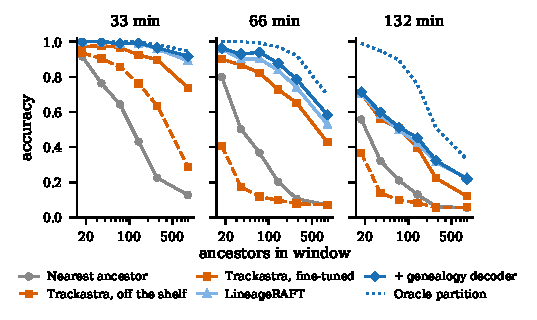
\includegraphics[width=\linewidth]{fig/density.pdf}
\caption{\textbf{Accuracy against colony size} on OIAM M3/M4 (windows binned by number of ancestors). Frame-to-frame methods collapse in dense colonies; family registration degrades gracefully, and the remaining gap to the oracle partition at long gaps is a grouping problem.}
\label{fig:density}
\end{figure}

\section{Biology read from two snapshots}
\cref{tab:downstream} computes from predicted ancestry two readouts a biologist would take from lineage: size control (longer ancestors divide sooner) and the spread of family sizes across ancestors, a measure of growth heterogeneity.
Nearest assignment destroys the first and inflates the second 1.7- to 3.2-fold; both \ours models are close to the ground truth at 33 minutes, and at 66 minutes keep a correlation of 0.7 between predicted and true family size.
\begin{table}[t]
\centering\small
\setlength{\tabcolsep}{3pt}
\begin{adjustbox}{max width=\linewidth}
\begin{tabular}{lccccccc}
\toprule
 & \multicolumn{3}{c}{Size control (33 min)} & \multicolumn{3}{c}{CV of family size} & $r(\hat n,n)$ \\
\cmidrule(lr){2-4}\cmidrule(lr){5-7}\cmidrule(lr){8-8}
Method & $\rho$ & long & short & 33 & 66 & 132 & 66 \\
\midrule
Ground truth & .574 & .789 & .003 & .369 & .314 & .496 & 1.000 \\
\midrule
Nearest ancestor & .134 & .341 & .211 & .620 & .919 & 1.567 & .069 \\
\rodsim only & .174 & .395 & .223 & .412 & .402 & .357 & .281 \\
\ours, self-labelled & .489 & .688 & .039 & .396 & .441 & .658 & .679 \\
\ours & .510 & .711 & .027 & .397 & .439 & .646 & .692 \\
\bottomrule
\end{tabular}
\end{adjustbox}
\caption{\textbf{Biology read from two snapshots} (OIAM M3/M4, 32 random windows per gap and movie). Family size $n$ is the number of descendants assigned to an ancestor. Size control: Spearman $\rho$ between ancestor length (ranked within window) and $n$, and the fraction of the longest and shortest third of ancestors that divided within 33 minutes. CV: coefficient of variation of $n$ across ancestors (growth heterogeneity). $r(\hat n,n)$: Pearson correlation of predicted with true family size at 66 minutes.}
\label{tab:downstream}
\end{table}


\section{Partition-aware decoding}
\cref{tab:decoder} gives every decoder setting for two base models. Larger $\beta$ helps at short and medium gaps but not on dense windows at 132 minutes, and hard clustering helps most at 132 minutes; $\beta{=}2$ is the setting reported in the main text. Both networks are trained on M0--M2, so no annotated movie is left to select it on; instead we cross-fitted the choice among $\beta\in\{1,2,4\}$ and Cluster\,+\,argmax, selecting on M3 and scoring M4 and vice versa. This gives equal or higher accuracy than fixed $\beta{=}2$ for every base model at every gap (three-seed ensemble 0.978/0.869/0.531 \vs 0.977/0.863/0.517; annotation-free pipeline without the consistency term, post hoc, 0.968/0.854/0.518 \vs 0.966/0.847/0.497), so the reported setting is not tuned to the test windows.
\begin{table}[t]
\centering\small
\setlength{\tabcolsep}{3.5pt}
\begin{adjustbox}{max width=\linewidth}
\begin{tabular}{llcccccc}
\toprule
& & \multicolumn{3}{c}{All} & \multicolumn{3}{c}{Dense} \\
\cmidrule(lr){3-5}\cmidrule(lr){6-8}
Model & Decoder & 33 & 66 & 132 & 33 & 66 & 132 \\
\midrule
No rot. & argmax & .849 & .653 & .447 & .717 & .443 & .247 \\
 & Potts $\beta{=}1$ & .873 & .688 & .458 & .763 & .488 & .248 \\
 & Potts $\beta{=}2$ & .890 & .706 & .462 & .786 & .506 & .240 \\
 & Potts $\beta{=}4$ & .902 & .729 & .461 & .799 & .505 & .229 \\
 & Cluster + argmax & .876 & .724 & .490 & .769 & .494 & .253 \\
 & \textcolor{gray}{Oracle partition} & .947 & .855 & .731 & .876 & .658 & .380 \\
\midrule
Full & argmax & .961 & .794 & .486 & .913 & .603 & .269 \\
 & Potts $\beta{=}1$ & .966 & .814 & .493 & .925 & .635 & .274 \\
 & Potts $\beta{=}2$ & .969 & .828 & .498 & .933 & .656 & .271 \\
 & Potts $\beta{=}4$ & .973 & .841 & .506 & .938 & .661 & .264 \\
 & Cluster + argmax & .955 & .830 & .526 & .926 & .649 & .274 \\
 & \textcolor{gray}{Oracle partition} & .982 & .911 & .764 & .958 & .777 & .418 \\
\bottomrule
\end{tabular}
\end{adjustbox}
\caption{\textbf{Partition-aware decoding} with single-snapshot genealogy on OIAM M3/M4. $\beta$ was not tuned on held-out data; all values are shown; the Darcy-initialised model behaves alike. Cluster + argmax: average-linkage clusters of the genealogy affinities cut at 0.3, each cluster sent to the ancestor with the largest summed log-probability. Full is training seed 0; the main results table applies Potts $\beta{=}2$ to the probability ensemble of three seeds. Decoding skips the one 33-minute window with fewer than nine target cells, which moves 33-minute argmax values by up to 0.009 from other tables.}
\label{tab:decoder}
\end{table}

Averaging the probabilities of the three training seeds helps the decoder more than any single model (0.057 \vs 0.034 at 66 minutes).
\cref{tab:calibration} suggests why: single models are overconfident (mean confidence 0.83 at 66 minutes for an accuracy of 0.60), and the ensemble's probabilities are better calibrated, so the genealogy prior can overrule confident mistakes.
\begin{table}[t]
\centering\small
\setlength{\tabcolsep}{4pt}
\begin{adjustbox}{max width=\linewidth}
\begin{tabular}{lccc}
\toprule
Gap & Accuracy & ECE & NLL of true ancestor \\
\midrule
33 min & 0.895 $\to$ 0.912 & 0.051 $\to$ 0.013 & 0.608 $\to$ 0.404 \\
66 min & 0.599 $\to$ 0.634 & 0.229 $\to$ 0.111 & 2.570 $\to$ 1.787 \\
132 min & 0.317 $\to$ 0.333 & 0.401 $\to$ 0.275 & 5.416 $\to$ 4.079 \\
\bottomrule
\end{tabular}
\end{adjustbox}
\caption{\textbf{Calibration} of the full model on OIAM M3/M4, pooled over scored targets: mean of three single seeds $\to$ their probability-averaged ensemble. ECE: expected calibration error of the top choice (15 bins). Single models are overconfident; averaging at least halves ECE at 33 and 66 minutes.}
\label{tab:calibration}
\end{table}

Is calibration the reason? We fitted one temperature per model and gap by the likelihood of the true ancestor on M0--M2 (protocol fixed before running) and decoded M3/M4 once (\cref{tab:temperature}).
Even on the movies they were trained on, the models are overconfident (fitted $T{=}1.6$--$1.8$ for single seeds, 1.3--1.4 for the ensemble). On M3/M4 the temperature cuts the single models' ECE at 66 minutes from 0.23 to 0.14 and raises their decoded accuracy at that gap with every seed (+0.010 to +0.014), recovering about half of the gap between the single-model and ensemble decoder gains (0.034 and 0.057 at 66 minutes).
It leaves the ensemble unchanged (within 0.004) and does not help dense windows at 132 minutes, so calibration explains part of the ensemble's advantage; the rest comes from its better base predictions.
\begin{table}[t]
\centering\small
\setlength{\tabcolsep}{4pt}
\begin{adjustbox}{max width=\linewidth}
\begin{tabular}{lcccccc}
\toprule
& \multicolumn{3}{c}{All windows} & \multicolumn{3}{c}{Dense} \\
\cmidrule(lr){2-4}\cmidrule(lr){5-7}
Probabilities $\to$ decoder & 33 & 66 & 132 & 33 & 66 & 132 \\
\midrule
Single seed, argmax & .955 & .780 & .473 & .907 & .598 & .267 \\
Single seed & .966 & .814 & .485 & .928 & .650 & .275 \\
Single seed, fitted $T$ & .969 & .826 & .489 & .934 & .660 & .269 \\
Ensemble, argmax & .964 & .807 & .490 & .923 & .634 & .284 \\
Ensemble & .976 & .863 & .516 & .946 & .703 & .300 \\
Ensemble, fitted $T$ & .977 & .867 & .515 & .947 & .705 & .296 \\
\bottomrule
\end{tabular}
\end{adjustbox}
\caption{\textbf{Temperature before decoding} (OIAM M3/M4; Potts $\beta{=}2$ unless argmax). $T$ is chosen per model and gap by the likelihood of the true ancestor on M0--M2 and applied once. Single-seed rows: mean of three seeds. Here each seed is normalised before averaging, which moves ensemble rows by at most 0.001 from the main table. Decoding skips the one 33-minute window with fewer than nine target cells, which moves 33-minute argmax values by up to 0.009 from other tables.}
\label{tab:temperature}
\end{table}

Seed averaging does not change the zero-shot picture: for the three \rodsim training seeds on the six datasets of the main transfer table, the ensemble is within $-0.004$ to $+0.011$ of seed 0 and $0.003$--$0.015$ above the seed mean, and it beats the best geometric baseline on exactly the same sequences.

\paragraph{Is the decoder specific to \ours?}
No. Under a protocol fixed before running (\texttt{docs/decoder\_on\_baselines\_protocol.md}) we applied the same decoder to fine-tuned Trackastra and to family-centre regression (\cref{tab:decbase}).
It lifts Trackastra by 0.05/0.07 at 33/66 minutes; at 132 minutes it helps with Trackastra's raw probabilities ($+$0.024) but hurts with the temperature fitted on M2 ($-$0.039), the pre-registered primary setting.
On GBDT's unaries it is worse than GBDT's own collective decoder, which already couples neighbours through learned geometric affinities.
All three hypotheses hold: decoded \ours beats decoded Trackastra at every gap ($+$0.029 [0.012, 0.049], $+$0.029 [0.006, 0.057], $+$0.073 [0.042, 0.103]) and decoded GBDT, and at 132 minutes the decoded ensemble beats both ($+$0.105 [0.077, 0.135] over Trackastra).
Against the better-decoding raw-probability variant the margins are $+$0.027/$+$0.025/$+$0.010, the last with a CI including zero ($-$0.024--0.044); the decoded ensemble leads by $+$0.042 [0.007, 0.078] and the annotation-free ensemble by $+$0.024/$+$0.032/$+$0.012 (CIs above zero at 33/66).
The long-gap advantage is therefore shared between the family-registration probabilities and the decoder, and at 132 minutes it needs the ensemble.
\begin{table}[t]
\centering\small
\setlength{\tabcolsep}{3pt}
\begin{adjustbox}{max width=\linewidth}
\begin{tabular}{llcccccc}
\toprule
 & & \multicolumn{3}{c}{All windows} & \multicolumn{3}{c}{Dense ($>$200)} \\
\cmidrule(lr){3-5}\cmidrule(lr){6-8}
Base & Decoding & 33 & 66 & 132 & 33 & 66 & 132 \\
\midrule
Trackastra, fine-tuned & argmax & .889 & .716 & .451 & .788 & .507 & .171 \\
 & + decoder, $T$ fitted on M2 & .937 & .785 & .412 & .869 & .586 & .151 \\
 & + decoder, $T{=}1$ & .939 & .789 & .475 & .873 & .601 & .169 \\
Family-centre regression & own geometric decoder & .717 & .602 & .441 & .452 & .289 & .201 \\
 & argmax & .602 & .494 & .380 & .390 & .263 & .168 \\
 & + decoder & .521 & .485 & .359 & .376 & .261 & .150 \\
\ours, full (3 seeds) & argmax & .955 & .780 & .473 & .907 & .598 & .267 \\
 & + decoder & .966 & .814 & .485 & .928 & .650 & .275 \\
\ours, 3-seed ensemble & + decoder & \textbf{.977} & \textbf{.863} & \textbf{.517} & \textbf{.946} & \textbf{.703} & \textbf{.300} \\
\bottomrule
\end{tabular}
\end{adjustbox}
\caption{\textbf{The genealogy decoder on baseline probabilities} (OIAM M3/M4, decoder windows; Potts $\beta{=}2$ on the same image affinities; protocol fixed before running). Trackastra: row-normalised association weights; GBDT: softmax of its own cost at its decoder temperature, and its own collective decoder with geometric affinities and capacity (the main-table setting).}
\label{tab:decbase}
\end{table}


\paragraph{Overlapping windows.}
Test windows start every 33 minutes and span up to 132, so neighbouring windows share frames and window-level CIs are optimistic.
Under a protocol fixed before computing (\texttt{docs/block\_bootstrap\_protocol.md}) we resampled blocks of four consecutive windows within each movie (\cref{tab:blockboot}).
The pre-registered hypothesis, that every comparison significant over windows stays significant over blocks, \textbf{fails}: 14 of 19 do.
Every margin at 33 and 66 minutes over fine-tuned Trackastra, the direct matcher and the regressor survives, as does the decoded ensemble's lead over Trackastra at 132 minutes.
No undecoded single-model margin at 132 minutes survives (lower bounds $-$0.005 to $-$0.002), nor do the decoder-on-decoder margins at 66 minutes; the annotation-free pipeline's lead at 132 minutes is positive in both movies ($+$0.022, $+$0.051) but its block CI touches zero.
Blocks of eight windows give the same picture.
\begin{table*}[t]
\centering\small
\setlength{\tabcolsep}{3pt}
\begin{adjustbox}{max width=\linewidth}
\begin{tabular}{lccccccccc}
\toprule
 & \multicolumn{3}{c}{33 min} & \multicolumn{3}{c}{66 min} & \multicolumn{3}{c}{132 min} \\
\cmidrule(lr){2-4}\cmidrule(lr){5-7}\cmidrule(lr){8-10}
Comparison & mean & windows & blocks of 4 & mean & windows & blocks of 4 & mean & windows & blocks of 4 \\
\midrule
Full $-$ Trackastra, fine-tuned & +0.065 & \textbf{+0.045, +0.087} & \textbf{+0.030, +0.087} & +0.064 & \textbf{+0.043, +0.087} & \textbf{+0.037, +0.085} & +0.023 & {-0.003, +0.048} & {-0.019, +0.046} \\
Full $-$ direct matcher & +0.101 & \textbf{+0.068, +0.138} & \textbf{+0.041, +0.138} & +0.096 & \textbf{+0.072, +0.123} & \textbf{+0.057, +0.123} & +0.017 & \textbf{+0.004, +0.031} & {-0.005, +0.028} \\
Full $-$ regressor (GBDT) & +0.226 & \textbf{+0.160, +0.297} & \textbf{+0.104, +0.331} & +0.170 & \textbf{+0.126, +0.214} & \textbf{+0.095, +0.249} & +0.027 & \textbf{+0.003, +0.048} & {-0.002, +0.057} \\
Ens.\ + dec.\ $-$ Trackastra, fine-tuned & +0.088 & \textbf{+0.063, +0.116} & \textbf{+0.041, +0.117} & +0.148 & \textbf{+0.123, +0.174} & \textbf{+0.113, +0.183} & +0.067 & \textbf{+0.041, +0.093} & \textbf{+0.032, +0.089} \\
No annotation $-$ Trackastra, fine-tuned & +0.074 & \textbf{+0.052, +0.098} & \textbf{+0.034, +0.097} & +0.106 & \textbf{+0.081, +0.131} & \textbf{+0.074, +0.135} & +0.036 & \textbf{+0.010, +0.064} & {-0.001, +0.054} \\
Full + dec.\ $-$ Trackastra + dec.\ (fitted $T$) & +0.029 & \textbf{+0.012, +0.049} & \textbf{+0.005, +0.041} & +0.029 & \textbf{+0.006, +0.057} & {-0.005, +0.049} & +0.073 & \textbf{+0.042, +0.103} & \textbf{+0.034, +0.106} \\
Full + dec.\ $-$ Trackastra + dec.\ ($T{=}1$) & +0.027 & \textbf{+0.011, +0.047} & \textbf{+0.005, +0.039} & +0.025 & \textbf{+0.002, +0.051} & {-0.007, +0.043} & +0.010 & {-0.024, +0.044} & {-0.043, +0.051} \\
\bottomrule
\end{tabular}
\end{adjustbox}
\caption{\textbf{Window \vs time-block bootstrap} (OIAM M3/M4; 95\% CIs of the mean paired difference in accuracy, bold when above zero). Blocks: four consecutive windows (132 minutes of anchor times) resampled within each movie. Full: mean of three seeds; ensemble, decoder and no-annotation rows on the decoder windows.}
\label{tab:blockboot}
\end{table*}


\paragraph{Grouping, scored directly.}
Ancestor accuracy mixes two errors: splitting or merging families, and naming the wrong ancestor for a correct family. \cref{tab:partition} scores grouping alone. The decoder's effect is mainly on grouping: for single models it raises pair family F1 by 0.05/0.10/0.04 but accuracy by only 0.01/0.03/0.01, and for the ensemble by 0.06/0.15/0.08 \vs 0.01/0.06/0.03; on dense windows at 66 minutes single-model F1 rises from 0.41 to 0.57. At 132 minutes a single \ours model groups barely better than the GBDT regressor (0.32 \vs 0.31) although it is more accurate; the decoded ensemble reaches 0.41.
\begin{table}[t]
\centering\small
\setlength{\tabcolsep}{3pt}
\begin{adjustbox}{max width=\linewidth}
\begin{tabular}{lccccccccc}
\toprule
 & \multicolumn{3}{c}{Accuracy} & \multicolumn{3}{c}{Pair family F1} & \multicolumn{3}{c}{F1, dense} \\
\cmidrule(lr){2-4}\cmidrule(lr){5-7}\cmidrule(lr){8-10}
Method & 33 & 66 & 132 & 33 & 66 & 132 & 33 & 66 & 132 \\
\midrule
Nearest ancestor & .484 & .361 & .263 & .277 & .238 & .209 & .078 & .091 & .102 \\
Family-centre regression (GBDT) & .717 & .602 & .441 & .541 & .459 & .309 & .265 & .192 & .190 \\
\ours (mean of three seeds) & .955 & .780 & .473 & .884 & .621 & .319 & .774 & .408 & .228 \\
\quad + genealogy decoder & .966 & .814 & .485 & .933 & .717 & .363 & .871 & .566 & .282 \\
\ours, 3-seed ensemble & .964 & .807 & .490 & .906 & .662 & .330 & .815 & .449 & .242 \\
\quad + genealogy decoder & .977 & .863 & .517 & .962 & .812 & .405 & .919 & .648 & .295 \\
\quad + decoder, no annotation & .963 & .822 & .487 & .941 & .756 & .394 & .881 & .577 & .262 \\
\bottomrule
\end{tabular}
\end{adjustbox}
\caption{\textbf{Grouping, scored directly} (OIAM M3/M4, windows with at least nine targets). Pair family F1 counts pairs of scored targets that share the true ancestor and are given the same ancestor, whichever it is; the adjusted Rand index agrees within 0.03. The oracle partition scores 1 by construction. GBDT is retrained on M0--M2 here, so its accuracy differs slightly from the main table.}
\label{tab:partition}
\end{table}


\paragraph{What limits the decoder?}
In a post hoc diagnostic on the three-seed ensemble we replaced the predicted affinities by true ones (1 if two neighbours share an ancestor $H$ minutes earlier, 0 otherwise) and widened the genealogy graph from 8 to 16 or 24 neighbours. With predicted affinities the wider graph changes accuracy by at most 0.004 at any gap. With true affinities it lifts 132-minute accuracy from 0.61 to 0.65 ($\beta{=}2$) and 0.70 ($\beta{=}4$, 24 neighbours), still below the 0.78 of the oracle partition (dense windows: at most 0.40 \vs 0.47). Potts mean field, however, is a weak partitioner even with true affinities. In a follow-up fixed in advance (\texttt{docs/global\_partition\_protocol.md}) we replaced it by non-local partitioners on 8- and 24-neighbour target graphs: correlation clustering of the affinity log-odds (greedy additive edge contraction with local moves), the same objective with \ours' co-assignment log-odds added, and spectral clustering with as many clusters as distinct argmax ancestors, each partition assigned to ancestors by Cluster\,+\,argmax or Hungarian matching. With predicted affinities none improves on Potts at 132 minutes (best 0.517 \vs 0.517, paired CI $-$0.014--0.014; dense 0.293 \vs 0.300; spectral 0.45), although pair family F1 rises from 0.41 to 0.47; at 66 minutes all are below Potts. With true affinities, correlation clustering on the 24-neighbour graph with Hungarian assignment reaches 0.780 (dense 0.454), the oracle partition's 0.784 (0.465). The remaining gap at long gaps is therefore the accuracy of single-image genealogy, not the locality of the decoder.

\section{Simulator ablation}
\cref{tab:simablate} retrains the positions-only \rodsim model with one ingredient changed and evaluates it zero-shot.
Removing physics randomisation or the field-of-view crop costs at most 0.02, and 16 simulated colonies are as good as 256, whereas randomising division modes (asymmetry, V-snapping) hurts transfer of the assignment model by about 0.05 (it helps the genealogy model, \cref{sec:supp-labelfree}).
What the network extracts from \rodsim is a simple prior on how growing rods push each other apart.
\begin{table}[t]
\centering\small
\setlength{\tabcolsep}{3pt}
\begin{adjustbox}{max width=\linewidth}
\begin{tabular}{lcccc}
\toprule
Simulator variant & FAST & recA & rpsM & OIAM \\
\midrule
Full \rodsim (256 colonies) & .712 & .566 & .571 & .525 \\
No physics randomisation & .701 & .552 & .562 & .521 \\
No field-of-view crop & .696 & .549 & .559 & .507 \\
64 colonies & .713 & .560 & .577 & .524 \\
16 colonies & .720 & .580 & .592 & .522 \\
+ division modes & .658 & .507 & .504 & .485 \\
\bottomrule
\end{tabular}
\end{adjustbox}
\caption{\textbf{Simulator ablations} (zero-shot accuracy, mean over gaps; every row is one training seed, seed 0, so it differs from the three-seed means of the zero-shot table).}
\label{tab:simablate}
\end{table}


\section{A pipeline without any real label}
\label{sec:supp-labelfree}
\cref{tab:labelfree} decodes the \rodsim-trained \ours with \rodsim-trained genealogy.
Genealogy with division modes improves every gap (up to 3 points), the symmetric simulator's does not; genealogy trained on real labels gains about three times as much.
\begin{table}[t]
\centering\small
\setlength{\tabcolsep}{4pt}
\begin{adjustbox}{max width=\linewidth}
\begin{tabular}{lccc}
\toprule
Genealogy in the decoder & 33 & 66 & 132 \\
\midrule
none (argmax) & .656 & .516 & .393 \\
\rodsim & .659 & .520 & .376 \\
\rodsim + division modes & .667 & .546 & .408 \\
OIAM M0--M2 labels & .696 & .597 & .434 \\
\textcolor{gray}{oracle partition} & .768 & .718 & .679 \\
\bottomrule
\end{tabular}
\end{adjustbox}
\caption{\textbf{A label-free pipeline.} \ours trained only on \rodsim, decoded with single-image genealogy from different sources (Potts, $\beta{=}1$); OIAM M3/M4 accuracy. The first three rows use no real label. Decoding skips the one 33-minute window with fewer than nine target cells, which moves 33-minute argmax values by up to 0.009 from other tables.}
\label{tab:labelfree}
\end{table}

Real images need not mean real labels: the genealogy network trained on chained pseudo-lineage of the unannotated M0--M2 movies (same links as the self-labelled assignment model; protocol fixed before training) agrees with the annotated pair labels on 94--100\% of pairs in sampled M0 frames (lowest for dense frames and long horizons) and reaches 0.96/0.89/0.69 AP on M3/M4 at 33/66/132 minutes (annotated: 0.97/0.91/0.70). Post hoc, the self-labelled assignment model without the consistency term (three seeds), decoded in the same way, reaches 0.966/0.847/0.497.
In the Potts decoder ($\beta{=}2$) it changes the accuracy of each full-model seed by at most 0.005 and of the three-seed ensemble by at most 0.003 (dense: 0.004) (0.976/0.861/0.520 \vs 0.977/0.863/0.517; dense 0.945/0.699/0.296 \vs 0.946/0.703/0.300).

\section{Robustness to detection errors}
\cref{fig:robustness} perturbs both snapshots of every OIAM M3/M4 window at the 33-minute gap with position noise, missed detections, merges of a cell with its nearest neighbour (under-segmentation) and spurious detections; only targets that survive unmerged and whose ancestor survives unmerged are scored.
With 10\% of cells missed, merged or hallucinated, \ours is still correct for 90--91\% of targets, against about 50\% for nearest assignment on the same targets.
Position noise of $0.3$ cell spacings, far beyond the localisation error of a modern segmenter, lowers accuracy to 0.82.
The ordering is unchanged at 66 and 132 minutes.
With Cellpose-SAM masks, the loss concentrates in the first, sparse frames, where a few spurious objects distort the population-size normalisation.

\paragraph{A second segmenter.}
\cref{tab:segmenters} adds Omnipose~\cite{cutler2022omnipose}, run with the settings of its official bacterial phase-contrast notebook under a protocol fixed before any test frame was segmented (one amendment: a dependency pin needed to import it). It finds every annotated cell but adds 16--43 small objects to every M3 frame, out-of-colony debris that Cellpose-SAM mostly ignores. On M4 the full model keeps 0.94/0.74/0.46 with Omnipose masks; on the small early M3 colonies the debris corrupts the population-size inputs ($N_a$, $N_b$, centroid, spacing) and accuracy falls below nearest assignment. Dense windows lose at most 0.08. We did not filter the debris, since any filter would be chosen on the test movies; a size or colony-membership filter is the obvious remedy and the population-size inputs are the component to harden.
\begin{table*}[t]
\centering\small
\setlength{\tabcolsep}{4pt}
\begin{tabular}{llcccccccc}
\toprule
 & & \multicolumn{2}{c}{Detection} & \multicolumn{3}{c}{All windows} & \multicolumn{3}{c}{Dense ($N_a{>}200$)} \\
\cmidrule(lr){3-4}\cmidrule(lr){5-7}\cmidrule(lr){8-10}
Model & Positions & Rec. & Prec. & 33 & 66 & 132 & 33 & 66 & 132 \\
\midrule
\ours & true & 1 & 1 & .957 & .780 & .473 & .907 & .598 & .267 \\
 & Cellpose-SAM & 1.000 & .936 & .922 & .730 & .436 & .902 & .592 & .262 \\
 & Omnipose & 1.000 & .852 & .736 & .503 & .287 & .877 & .522 & .220 \\
\midrule
\ours, no annotation & true & & & .935 & .733 & .452 & .865 & .533 & .244 \\
 & Cellpose-SAM & & & .918 & .697 & .420 & .859 & .531 & .243 \\
 & Omnipose & & & .749 & .500 & .281 & .843 & .489 & .207 \\
\midrule
\ours, \rodsim only & true & & & .657 & .512 & .390 & .333 & .197 & .096 \\
 & Cellpose-SAM & & & .562 & .438 & .342 & .342 & .201 & .099 \\
 & Omnipose & & & .486 & .355 & .230 & .332 & .195 & .104 \\
\midrule
Nearest ancestor & true & & & .497 & .361 & .263 & .157 & .083 & .058 \\
 & Cellpose-SAM & & & .497 & .359 & .261 & .155 & .081 & .055 \\
 & Omnipose & & & .495 & .360 & .259 & .156 & .080 & .047 \\
\bottomrule
\end{tabular}
\caption{\textbf{End-to-end with two off-the-shelf segmenters} on OIAM M3/M4, neither fine-tuned nor tuned (Cellpose-SAM; Omnipose \texttt{bact\_phase\_omni} with the settings of its official notebook, fixed before segmenting). Accuracy is correct over \emph{all} annotated targets (missed or mismatched cells count as errors), mean of three training seeds. Both segmenters find essentially every cell; losses come from spurious objects, under Omnipose mostly out-of-colony debris in the sparse early frames of M3, so dense windows lose at most 0.08.}
\label{tab:segmenters}
\end{table*}

\begin{figure*}[t]
\centering
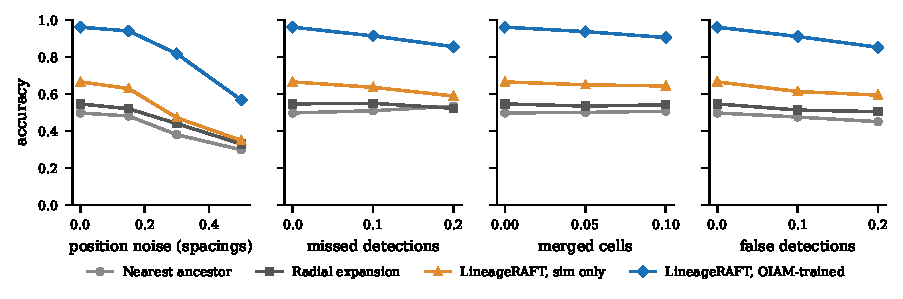
\includegraphics[width=0.8\linewidth]{fig/robustness.pdf}
\caption{\textbf{Robustness to detection errors} on OIAM M3/M4 at a 33-minute gap. Each perturbation is applied independently to both snapshots; the leftmost point of every panel is the unperturbed result.}
\label{fig:robustness}
\end{figure*}

\section{Self-labelling details}
\paragraph{Linking.}
One-frame links are solved with \texttt{scipy}'s exact linear assignment over the $8$ nearest slots of each target.
On OIAM (masks available) the daughter slots sit at $\pm L/4$ along the mother's axis, with $L=\sqrt{12}$ times the major-axis standard deviation of the mask; the extra division cost is 10\,px and the no-parent cost 60\,px (0.55 and 3.5 median spacings).
For the external sources, which provide positions only, both daughter slots sit at the mother's centre and costs are scaled by the median spacing of each frame.
These values were set on OIAM M0 and never tuned on the external sources.

\paragraph{Does self-labelling need family registration?}
Under a protocol fixed before training (\texttt{docs/pseudo\_direct\_matcher\_protocol.md}) we trained the direct matcher (frozen family centre) on the same pseudo-lineage, recipe and seeds as self-labelled \ours. Both pre-registered hypotheses hold. Self-labelling is not specific to \ours: it costs the direct matcher only 0.009/0.011/0.012 (0.847/0.673/0.444 \vs 0.856/0.684/0.456 on true lineage). The architecture margin survives it: self-labelled \ours leads the self-labelled direct matcher by 0.088 [0.058, 0.122] and 0.059 [0.037, 0.082] at 33/66 minutes (0.008 [$-$0.005, 0.021] at 132; dense 0.865/0.533/0.244 \vs 0.686/0.412/0.199), and even the direct matcher trained on true lineage by 0.079 and 0.048 (CIs above zero). In domain, family registration with no annotation thus beats cell matching with annotation at 33 and 66 minutes.

\paragraph{Quality of pseudo-lineage.}
\cref{tab:pseudo} reports the fraction of cells whose chained ancestor equals the annotated one.
Errors at divisions dominate without the fission prior: on M0, one-frame links are wrong for 30\% of dividing mothers and 0.5\% of the others; the daughter slots reduce the former to 4\%.
Because a swap between two sisters does not change ancestry at longer gaps, the composed accuracy decays slowly with $H$.

\begin{table}[t]
\centering\small
\setlength{\tabcolsep}{4pt}
\begin{tabular}{lcccc}
\toprule
Data (gap) & 33/30 & 66/60 & 132/120 & 240 \\
\midrule
OIAM M0, fission prior & .977 & .930 & .921 & .927 \\
OIAM M0, no daughter slots & .844 & .700 & .570 & .522 \\
OIAM M1 & .976 & .930 & .929 & .928 \\
OIAM M2 & .910 & .912 & .893 & .881 \\
\midrule
\emph{B.\ subtilis} (positions only) & .976 & .968 & .927 & -- \\
LYN yeast & .950 & .914 & .852 & -- \\
TrackMate & .892 & .834 & .869 & -- \\
TrackRefiner & .739 & .654 & .551 & -- \\
\bottomrule
\end{tabular}
\caption{\textbf{Accuracy of chained pseudo-lineage} against the annotation, weighted by cells, over random windows (minutes; OIAM at 33/66/132/240, external sources at 30/60/120). TrackRefiner movies are sampled every 2 minutes with large motion between frames.}
\label{tab:pseudo}
\end{table}

\paragraph{Protocol 3.}
The protocol (\texttt{docs/blind\_test3\_protocol.md}) fixed, before training: two folds per source by sorted sequence name; 6k fine-tuning steps from the \rodsim model at learning rate $2{\times}10^{-4}$, positions only, horizons log-uniform in 15--240 minutes; evaluation on the windows of blind tests 1 and 2 with the same seeds.
One amendment was made before any evaluation: some short \emph{B.\ subtilis} sequences admit no frame pair at long horizons, so the sampler draws another sequence when 100 draws fail.
Hypotheses and outcomes:
A1 (SV with the adapted model beats the best of eight geometric baselines) holds on TrackRefiner, TrackMate and LYN and fails on \emph{B.\ subtilis} (0.894 \vs 0.895);
A2 (it beats SV without adaptation) holds on TrackRefiner, LYN and \emph{B.\ subtilis} and fails on TrackMate (0.803 \vs 0.838);
A3 (the adapted whole-field model beats the \rodsim model) holds on all four.

\paragraph{Protocols 4 and 5.}
On FAST, recA and rpsM (\texttt{docs/selflabel\_ext\_protocol.md}), the same procedure with positions-only Hungarian links failed: adaptation was below the \rodsim model on every dataset and all 25 colonies (\cref{tab:bootstrap}).
Measured afterwards against the ground truth, one-frame Hungarian links are only 0.55 (recA), 0.84 (rpsM) and 0.94 (FAST) correct at these frame rates, and compose to 0.24--0.68, below the \rodsim model's direct accuracy; one-frame argmax links of the \rodsim model itself are 0.73, 0.94 and 0.99 correct.
Protocol 5 (\texttt{docs/selflabel\_bootstrap\_protocol.md}), fixed before training and run once, changes only the one-frame links to the \rodsim model's predictions; it is post hoc in that the data had been scored.
Both hypotheses hold on all three datasets: bootstrapping beats the \rodsim model (C1) and the best geometric baseline (C2).
\begin{table}[t]
\centering\small
\setlength{\tabcolsep}{4pt}
\begin{adjustbox}{max width=\linewidth}
\begin{tabular}{lccccc}
\toprule
Dataset & Best geom. & \rodsim & + Hungarian & + bootstrap & wins \\
\midrule
FAST & .593 & .702 & .642 & \textbf{.730} & 6/7 \\
recA & .466 & .563 & .445 & \textbf{.576} & 6/9 \\
rpsM & .455 & .560 & .450 & \textbf{.604} & 9/9 \\
\bottomrule
\end{tabular}
\end{adjustbox}
\caption{\textbf{Temporal bootstrapping} on the microcolony datasets (accuracy, mean over colonies of the mean over gaps; two folds per dataset, each model evaluated on the other fold). The \rodsim model is fine-tuned on pseudo-lineage chained from positions-only Hungarian links (protocol 4) or from its own one-frame predictions (protocol 5). Wins: colonies on which bootstrapping beats the \rodsim model.}
\label{tab:bootstrap}
\end{table}


\paragraph{Protocol 6.}
We then applied bootstrapping to the four blind sources of protocol 3 (\texttt{docs/selflabel\_bootstrap\_blind\_protocol.md}; same folds, windows and settings), again fixed before training and run once.
E1 (the bootstrapped whole-field model beats the Hungarian-adapted one) fails on all four sources: 0.405 \vs 0.478 on TrackRefiner, 0.549 \vs 0.704 on TrackMate, 0.846 \vs 0.849 on yeast and 0.885 \vs 0.887 on \emph{B.~subtilis}.
E2 (SV with the bootstrapped model beats the best geometric baseline) holds on TrackRefiner (0.559 \vs 0.461), TrackMate (0.832 \vs 0.796) and yeast (0.858 \vs 0.827) and fails on \emph{B.~subtilis} (0.894 \vs 0.895).
E3 (it beats SV with Hungarian adaptation) holds on TrackRefiner, TrackMate and yeast by 0.002--0.029 and fails on \emph{B.~subtilis} (0.8937 \vs 0.8942).
A likely reason, tested below: on these fields of many small colonies the whole-field \rodsim model is itself poor (0.30 on TrackRefiner), so its one-frame links are a worse teacher than Hungarian links, whereas on FAST, recA and rpsM it was the stronger of the two.
Bootstrapping is therefore useful when the teacher is reliable, which can be checked without labels only indirectly.

\paragraph{Can the teacher be judged without labels?}
A further protocol (\texttt{docs/teacher\_reliability\_protocol.md}), fixed before computing, measured six label-free statistics of the \rodsim teacher's one-frame links on every sequence that supplied pseudo-labels (114 sequences or colonies of the ten sources): mean top-1 probability, entropy, agreement with Hungarian links (primary), fraction of ancestors with descendants, agreement with nearest assignment, and a fission-aware cycle consistency. All six track the teacher's own link accuracy (Spearman $|\rho|$ 0.70--0.90; primary 0.84, 95\% CI 0.74--0.90), but none decides whether bootstrapping beats Hungarian self-labelling: no single threshold on the source mean of the primary statistic separates the six sources where it won from the four where it lost (best: 2 of 10 wrong), and the same holds for the other five. With ground truth the rule is simple: bootstrapping won exactly where the teacher's one-frame links are more accurate than Hungarian links (all ten sources). On TrackRefiner and TrackMate they are not (0.78 \vs 0.96 and 0.83 \vs 0.98), confirming the explanation above; on yeast and \emph{B.~subtilis} both are 0.99. Agreement is symmetric and cannot tell which linker is wrong. A rule combining teacher confidence and agreement separates all ten sources but was found after seeing them and is untested.

\section{Blind tests 1 and 2, per-colony processing and self-labelled adaptation}
\label{sec:supp-blind12}
All datasets above were inspected during development, so we fixed a protocol (data, gaps, models, baselines, metric, hypotheses) before running anything on 11 unseen sequences: eight TrackRefiner ground-truth movies~\cite{ahmadi2025trackrefiner} and three curated TrackMate \emph{E.\ coli} movies~\cite{anselmet2026trackmate}.
The single run failed (\cref{tab:blind}, left): the \rodsim-trained model loses to the best geometric baseline on both sources and wins on only 2 of 11 sequences, the only two that show a single colony.
The other fields hold 8 to 70 separate microcolonies or are steady-state chambers that flush cells out, so descendants do not move radially as \ours assumes.

\paragraph{Per-colony processing and label-free selection.}
From this diagnosis, ancestors are split into colonies by single linkage at three cell spacings, each target joins the colony of its nearest ancestor, and every colony is a separate input.
Since no single method is best everywhere (registration wins in crowded, expanding colonies, nearest assignment where cells barely move), we pick per input between nearest assignment and per-colony \ours using a biological consistency check: in a growing population every ancestor has at least one descendant, so we keep the hypothesis under which more anchors receive a target (ties: more uniform family sizes).
This survival-based selection (\ours-SV) is within 0.005 of a per-window oracle choice of its components on the first blind set, post hoc.

\paragraph{Second blind test.}
A second protocol, fixed before downloading the data, tested SV on six budding-yeast colonies from LYN~\cite{zelic2026lyn}, a different kingdom with asymmetric division, and 44 mostly sparse \emph{B.\ subtilis} spore-outgrowth sequences~\cite{kunzmann2026bsub}.
On yeast SV beats every geometric variant (0.842 \vs 0.827) but on only half of the colonies; on \emph{B.\ subtilis}, where most spores neither move nor divide, it is 0.008 below nearest assignment (0.895), failing all three hypotheses.

\paragraph{Self-labelled adaptation.}
Before adapting, we fixed a third protocol on the same windows (not blind, since the data had been scored): within each source, sequences are split into two folds, the \rodsim model is fine-tuned for 6k steps on positions-only pseudo-lineage of one fold, and evaluated on the other.
Adaptation improves the whole-field model on all four sources (\cref{tab:blind}, bottom), most where simulation failed: from 0.31 to 0.48 on TrackRefiner and from 0.42 to 0.70 on TrackMate.
With SV it beats the best geometric baseline on TrackRefiner (0.555 \vs 0.461, all 8 sequences), TrackMate and yeast, but not on \emph{B.~subtilis} (0.894 \vs 0.895).
On the microcolony datasets of the zero-shot table (FAST, recA, rpsM), Hungarian links are poor at their frame rates and adaptation hurts on all 25 colonies; with temporal bootstrapping, fixed in a further protocol, it beats the \rodsim model on all three datasets and 21 colonies, but not Hungarian self-labelling on the four blind sources (below).

\begin{table}[t]
\centering\small
\setlength{\tabcolsep}{3pt}
\begin{adjustbox}{max width=\linewidth}
\begin{tabular}{lcccc}
\toprule
 & \multicolumn{2}{c}{Blind test 1} & \multicolumn{2}{c}{Blind test 2} \\
\cmidrule(lr){2-3}\cmidrule(lr){4-5}
Method & TrackRefiner & TrackMate & LYN (yeast) & \emph{B.\ subtilis} \\
\midrule
Nearest ancestor & .407 & .796 & .827 & .895 \\
Best of 8 geometric & .461 & .796 & .827 & .895 \\
\ours, whole field & .306 & .419 & .817 & .874 \\
\ours, per colony & .501$^\dagger$ & .661$^\dagger$ & .828 & .878 \\
\ours-SV (label-free selection) & .496$^\dagger$ & .838$^\dagger$ & .842 & .887 \\
SV wins / sequences & 6/8$^\dagger$ & 3/3$^\dagger$ & 3/6 & 9/44 \\
\midrule
\multicolumn{5}{l}{\emph{+ self-labelling on the other fold's unannotated sequences (protocol 3)}} \\
\ours, whole field & .478 & .704 & .849 & .887 \\
\ours, per colony & .560 & .753 & .856 & .890 \\
\ours-SV & .555 & .803 & .856 & .894 \\
SV wins / sequences & 8/8 & 2/3 & 4/6 & 22/44 \\
\bottomrule
\end{tabular}
\end{adjustbox}
\caption{\textbf{Pre-registered blind tests and self-labelled adaptation.} Accuracy averaged over windows, gaps (30/60/120 min) and sequences; \rodsim-trained, positions only. Test 1 (11 sequences) was run first and failed; $^\dagger$per-colony processing and SV were designed after seeing it, so these test-1 entries are post hoc (SV there uses one seed). Test 2 (6 yeast colonies, 44 \emph{B.\ subtilis} sequences) was fixed before its data were downloaded and run once. Best of 8 geometric: nearest, centroid translation, radial expansion and radial sector (the ancestor in the most similar direction from the colony centroid), each on the whole field or per colony, best chosen per source after the run. Protocol 3 (not blind: same windows, method fixed before running) fine-tunes the \rodsim model on chained pseudo-lineage of the other half of each source's sequences, with no ground-truth lineage.}
\label{tab:blind}
\end{table}


\section{Blind-test protocols}
\Cref{tab:ledger} lists every protocol fixed before running, with its outcome.
\begin{table*}[t]
\centering\footnotesize
\setlength{\tabcolsep}{4pt}
\begin{tabular}{>{\raggedright\arraybackslash}p{2.6cm}>{\raggedright\arraybackslash}p{3.6cm}>{\raggedright\arraybackslash}p{5.4cm}>{\raggedright\arraybackslash}p{4.6cm}}
\toprule
Protocol & Data & Hypotheses (fixed before running) & Outcome (run once, reported as is) \\
\midrule
Blind test 1 & TrackRefiner, TrackMate; 11 seq., unseen & H1 \rodsim $>$ best geometric, per source; H2 on most sequences; H3 \rodsim $>$ OIAM-trained & H1 \textbf{fails} 0/2; H2 \textbf{fails} (2/11); H3 holds 2/2 \\
Blind test 2 & LYN yeast, \emph{B.~subtilis}; fixed before download & H1 SV $>$ best geometric; H2 on most sequences; H3 SV $\ge$ both components & yeast: H1, H3 hold, H2 fails (3/6); \emph{B.~subtilis}: all \textbf{fail} (9/44) \\
Protocol 3 & four blind-test sources, already scored; two folds & A1 adapted SV $>$ best geometric; A2 $>$ unadapted SV; A3 adapted $>$ \rodsim & A1 3/4; A2 3/4; A3 4/4 \\
Protocol 4 & FAST, recA, rpsM (not blind) & B1 Hungarian self-labelling $>$ \rodsim; B2 $>$ best geometric & B1 \textbf{fails} 0/3; B2 1/3 \\
Protocol 5$^\ddagger$ & FAST, recA, rpsM (not blind) & C1 bootstrapping $>$ \rodsim; C2 $>$ best geometric & C1 3/3; C2 3/3 \\
Protocol 6 & as protocol 3 & E1 bootstrapping $>$ Hungarian self-labelling; E2 its SV $>$ best geometric; E3 $>$ SV with Hungarian & E1 \textbf{fails} 0/4; E2 3/4; E3 3/4 \\
Blind test 4 & trpL, metA, pheA; 28 colonies, fixed before download & F1 \rodsim $>$ best of six baselines; F2 on most colonies; F3 bootstrapping $>$ \rodsim; F4 $>$ Hungarian & all hold, 3/3 subsets, every gap \\
Teacher reliability & ten self-labelling sources, 114 units & (a) label-free teacher statistics track one-frame link accuracy; (b) primary statistic separates sources where bootstrapping wins & (a) holds ($\rho{=}0.84$); (b) \textbf{fails} (2/10 wrong) \\
Matched direct matcher & OIAM M3/M4; 80k steps, 3 seeds per arm & D1 \ours $>$ direct matcher (Darcy) every gap; D2 dense; D3 radial init. & D1, D2 hold (CIs $>$0); D3 \textbf{fails} at 132 min (tie) \\
Trackastra without rot.\ aug. & OIAM M3/M4; batch 8 (amended after a batch-16 run) & R1 no-rot.\ fine-tuning helps Trackastra at $\ge$2 gaps; R2 \ours $>$ better Trackastra at 33/66; R3 decoded ensemble $>$ it at all gaps & R1 \textbf{fails} (1/3); R2, R3 hold \\
Full-model LOMO & five OIAM folds, 80k steps, one seed & L1 $>$ no-rot.\ 30k at 33/66 on $\ge$4/5 folds; L2 $>$ regressor at every gap on $\ge$4/5; L3 mean $\ge$0.90 at 33 & all hold (5/5, 5/5; 0.954) \\
Centre controls & OIAM M3/M4; 80k steps, 3 seeds per arm & K1 \ours $>$ direct matcher with 96 candidates; K2 $>$ centre loss without moving; K3 $T{=}4 > T{=}1$ & all hold (CIs $>$0 at 33/66 min) \\
Orientation & OIAM M3/M4 in 8 image frames; estimator chosen on M0--M2 & H1 no correction worse; H2 primary rule recovers $\ge$75\% of the no-rotation gain; H3 per-window $<$ per-sequence; H4 confidence $>$ averaging & H1 holds; H2 holds at 33/66 (nothing to recover at 132); H3 mixed; H4 \textbf{fails} \\
Decoder on baselines & OIAM M3/M4, decoder windows & G1 decoded \ours $>$ decoded Trackastra at every gap (CI $>$0 at 33/66); G2 $>$ decoded GBDT; G3 decoded ensemble $>$ both at 132 & all hold; \vs raw-probability Trackastra $+$0.010 at 132 (CI includes 0) \\
Time-block bootstrap & OIAM M3/M4, 7 main comparisons & B1 every window-significant margin stays significant with blocks of 4 windows & \textbf{fails}: 14/19; 132-min single-model margins and 66-min decoder-on-decoder lost \\
Optical flow & OIAM; RAFT setting chosen on M0--M2 (8 settings) & R1 \ours $>$ flow at every gap; R2 flow $>$ nearest at 33 min & both hold (flow 0.636/0.367/0.244) \\
Trackastra zero-shot & FAST (images + corrected masks), 7 colonies & Z1 \rodsim-trained \ours $>$ Trackastra; Z2 on $\ge$5/7 colonies & both hold (0.709 \vs 0.626; 7/7) \\
\rodsim direct matcher & zero-shot table, 4 bacterial + 2 human datasets; 3 seeds (rerun at half lr after divergence) & S1 \ours $>$ direct matcher on all 4 bacterial datasets; S2 direct matcher $>$ best baseline on $\ge$3/4 & S1 \textbf{fails} (2/4: OIAM, FAST); S2 holds (4/4) \\
Matched Trackastra & OIAM M3/M4; \ours on M0/M1, 20k steps, 3 seeds; Trackastra over 5 gaps & M1/M2 matched \ours $>$ per-gap / multi-gap Trackastra at 33/66; M3 $\ge$ selected Trackastra at 132 & all \textbf{fail} (0.715/0.554/0.394); multi-gap Trackastra replaces the 132-min entry (0.488) \\
Direct matcher, van Vliet & 28 colonies of blind test 4; bootstrapped self-labelling, 6k steps & V1 \ours $>$ direct matcher over colonies (CI $>$ 0); V2 in every subset & V1 fails ($+$0.003 [$-$0.001, 0.007]); V2 holds \\
Self-labelled direct matcher & OIAM M3/M4; pseudo-lineage of M0--M2, 80k steps, 3 seeds & P1 self-labelled \ours $>$ self-labelled direct matcher at 33/66; P2 self-labelling costs the direct matcher $<$0.05 & both hold ($+$0.088/$+$0.059; cost 0.01) \\
\midrule
Global partitioners & OIAM M3/M4, 66/132 min & no threshold; correlation and spectral clustering \vs Potts & predicted affinities: no gain (0.517 \vs 0.517); true: 0.780 \vs oracle 0.784 \\
Self-labelled genealogy & OIAM M3/M4 & no threshold; ensemble decoder \vs annotated genealogy & 0.976/0.861/0.520 \vs 0.977/0.863/0.517 \\
Annotation-free pipeline & OIAM M3/M4 & no threshold; full model on pseudo-lineage, 3 seeds & 0.963/0.822/0.487; no-consistency variant post hoc \\
Fine-tuned Trackastra & OIAM; trained on M0/M1, selected on M2 & no threshold; one model per gap, decoding fixed on M2 & 0.892/0.716/0.451 (\ours 0.957/0.780/0.473) \\
Lineage audit & recA, rpsM \vs curated FAST & no threshold; descriptive label statistics & flagged targets 5.2\%/1.7\% \vs 0.2\% (correction post hoc) \\
Second segmenter & Omnipose on OIAM M3/M4, notebook settings & no threshold; end-to-end accuracy & 0.74/0.50/0.29 (\vs 0.92/0.73/0.44 Cellpose-SAM); dense loss $\le$0.08 \\
Temperature scaling & OIAM; $T$ fitted on M0--M2 & no threshold; decoded once on M3/M4 & single seeds $+$0.010--0.014 at 66 min; ensemble unchanged \\
Structured decoder & OIAM M4 (M3 for development); FAST, recA, rpsM & vs Potts at 66/132: H1 lower size error and singleton rate; H2 pair F1; H3 accuracy not lower; H4 external: lower size error than argmax, accuracy not lower on $\ge$2/3 & H1, H2 hold; H3 holds at 66, \textbf{fails} at 132; H4 \textbf{fails} (accuracy 0/3) \\
Error decomposition & OIAM M3/M4 & no threshold; decision rule: largest error class on dense 132-min windows picks the next module & largest class needs both oracles (0.28 of errors); centre and partition tie \\
Coupled refinement & dev.\ M0/M1$\to$M2; then OIAM M3/M4, 80k steps, 3 seeds per arm & C1 coupled $>$ \ours every gap; C2 dense at 66/132; C3 lower centre error; C4 pair F1 at 132 & C1 \textbf{fails}; C2--C4 hold (C4 CI includes 0) \\
\rodsim v3 & OIAM M3/M4 zero-shot; FAST, recA, rpsM; 3 seeds per arm, equal lr & V1 v3 $>$ v1; V2 dense; V3 v3 \ours $>$ v3 direct matcher, dense; V4 no harm external & V1, V2 \textbf{fail}; V3, V4 hold \\
Midpoint snapshot & OIAM M3/M4, 66/132 min & A1 chaining through a midpoint $>$ direct at 132; A2 confidence policy recovers $\ge$75\% of the gain with half the snapshots & A1 holds ($+$0.235); A2 \textbf{fails} at 132 (51\%), 79\% at 66 \\
Growth heterogeneity & OIAM M3/M4 decoder windows, existing predictions & B1 decoded ensemble: lower error of family-size CV than decoded Trackastra and nearest at 66/132; B2 higher family-size rank correlation; B3 B1 without annotation & all hold (CIs $<$0 / $>$0); CV still 55\% too high at 132 min \\
\bottomrule
\end{tabular}
\caption{\textbf{Protocol ledger.} Every evaluation whose protocol was fixed in advance (files in \texttt{docs/}), in the order run; counts are sources, datasets or subsets on which a hypothesis holds. Failures are kept in the paper and drove the next protocol: per-colony processing and SV after test 1, bootstrapping after protocol 4. $^\ddagger$Post hoc in that the data had been scored before. Earlier protocols on recA and rpsM for a previous gradient-boosting method were invalidated by a coordinate bug found after scoring; all recA and rpsM results here are therefore development results, not blind.}
\label{tab:ledger}
\end{table*}

\paragraph{Blind test 2.}
The protocol (\texttt{docs/blind\_test2\_protocol.md}) was fixed before the LYN and \emph{B.~subtilis} data were downloaded and run once with the positions-only \rodsim model.
Hypotheses, per source: H1, SV beats the best of eight geometric variants (chosen per source after the run); H2, it does so on most sequences; H3, SV is at least as accurate as both of its components (nearest assignment and per-colony \ours).
On yeast H1 and H3 hold (0.842 \vs 0.827 and 0.828) and H2 fails (3 of 6 colonies); on \emph{B.~subtilis} all three fail (0.887 \vs 0.895; 9 of 44 sequences).

\paragraph{Blind test 4.}
The protocol (\texttt{docs/blind\_test4\_protocol.md}) was fixed before any file of the trpL, metA and pheA subsets of~\cite{vanvliet2018spatially} was downloaded; only the archive listings, which give colony names, were read.
It fixed all colonies with Schnitzcells lineage (10, 9 and 9), the 7.5-minute frame interval stated in that paper, gaps of 4, 8 and 16 frames, the recA window sampler and seed, six baselines (four geometric; exact and unbalanced OT without alignment at the OIAM-selected settings), the \rodsim model, and Hungarian and bootstrapped self-labelling with protocol-3 settings and folds by sorted colony rank.
Hypotheses, per subset: F1, \rodsim beats the best baseline; F2, on more than half of the colonies; F3, bootstrapping beats \rodsim; F4, bootstrapping beats Hungarian self-labelling.
One amendment was made before any window was scored: nine frames (in seven colonies) store an empty crop rectangle that the parser rejects; they are dropped and logged, and windows ending on them do not exist. No colony was excluded.
All hypotheses hold on all subsets (main-text table), at every gap: \rodsim exceeds the best baseline by 0.11--0.14 at 30 minutes and 0.06--0.09 at 120 minutes, and bootstrapping adds a further 0.03--0.06 at every gap.
\begin{figure}[t]
\centering
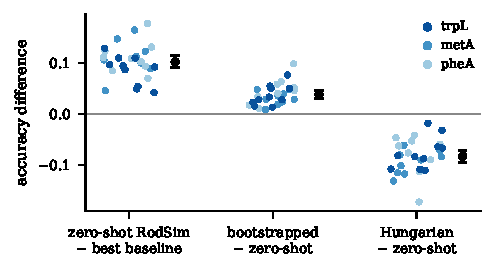
\includegraphics[width=\linewidth]{fig/blind4_effects.pdf}
\caption{\textbf{Blind test 4, colony by colony} (28 colonies, accuracy averaged over the three gaps). Left: the zero-shot \rodsim model minus the best of the six baselines \emph{for that colony}: positive on 28/28, mean $+0.102$ (95\% bootstrap CI over colonies 0.091--0.114). Middle: bootstrapped self-labelling minus zero-shot: 28/28, $+0.039$ (0.031--0.046). Right: Hungarian self-labelling minus zero-shot: negative on 28/28, $-0.083$ ($-0.095$ to $-0.071$). Black: mean and CI.}
\label{fig:blind4}
\end{figure}

\section{Where do long-gap errors go?}
For every wrong target in 24 random windows per gap and movie of OIAM M3/M4 we measured how long before the first snapshot the lineages of the predicted and the true ancestor split.
If errors at long gaps were confusions between sisters born just before the first snapshot, they would be an identifiability limit.
They are not: at 132 minutes only 6\% of \ours's errors confuse ancestors that split within 33 minutes, and 19\% within 132 minutes; forgiving all confusions between ancestors that split within 66 minutes raises cell-weighted accuracy only from 0.33 to 0.40.
The predicted ancestor is instead a neighbour of the true one, a median of 1.8 cell spacings away (nearest assignment: 3.6).
The residual error at long gaps is therefore a registration error of one to two cells, which is consistent with the oracle-partition result: knowing which cells form a family places most families correctly.
Feeding the predicted family centres back as the initialisation for a second pass does not refine them; it lowers accuracy at every gap (0.33 to 0.19 at 132 minutes), because the network learned offsets relative to the Darcy initialisation.

\section{Further negative results}
\paragraph{More refinement steps.}
Doubling the refinement rounds of the full model to $T{=}8$ (unshared weights, otherwise identical, 80k steps, one seed) lowers accuracy at every gap: 0.94/0.75/0.44 \vs 0.96/0.79/0.49 for $T{=}4$ (seed 0), and 0.88/0.58/0.24 \vs 0.91/0.60/0.27 on dense windows, although its final training accuracy is the same (0.96).
Consistent with the long-gap analysis above, the residual error is not resolved by iterating the same local update longer.

\paragraph{Fission-prior decoding.}
Replacing argmax by an exact MAP assignment under a log-normal prior on family size around $N_B/N_A$ (min-cost matching over ancestor slots with convex costs) changes accuracy by at most 0.01 (full model: 0.794$\to$0.800 at 66 minutes): predicted family sizes are already about right, and errors come from which cells form a family.

\paragraph{Forward simulation.}
FSA initialises \rodsim with the first snapshot (doubling time $H\ln 2/\ln(N_B/N_A)$), simulates $H$ minutes eight times, warps each rollout onto the second snapshot and assigns every target to the ancestor whose simulated descendants are densest there.
FSA's alignment by a similarity transform gives 0.60/0.51/0.38 on OIAM; a smooth non-rigid warp raises it to 0.63/0.53/0.39 and dropping the similarity step to 0.68/0.55/0.40.
These rollouts start from the true cell lengths and orientations; from positions only, as in the transfer experiments, FSA gives 0.57/0.45/0.36. With shapes (mean 0.54) it is the only baseline above the positions-only \rodsim model on OIAM (0.52); the other datasets lack comparable shape features.
Selecting rollouts by Chamfer distance to the second snapshot, or calibrating the doubling time so that the simulated count \emph{inside the field of view} matches $N_B$, does not help on dense windows (0.52/0.29/0.14 \vs 0.54/0.30/0.14).

{
    \small
    \bibliographystyle{ieeenat_fullname}
    \bibliography{main}
}
\end{document}
